% Options for packages loaded elsewhere
\PassOptionsToPackage{unicode}{hyperref}
\PassOptionsToPackage{hyphens}{url}
\documentclass[
]{article}
\usepackage{xcolor}
\usepackage[margin=1in]{geometry}
\usepackage{amsmath,amssymb}
\setcounter{secnumdepth}{-\maxdimen} % remove section numbering
\usepackage{iftex}
\ifPDFTeX
  \usepackage[T1]{fontenc}
  \usepackage[utf8]{inputenc}
  \usepackage{textcomp} % provide euro and other symbols
\else % if luatex or xetex
  \usepackage{unicode-math} % this also loads fontspec
  \defaultfontfeatures{Scale=MatchLowercase}
  \defaultfontfeatures[\rmfamily]{Ligatures=TeX,Scale=1}
\fi
\usepackage{lmodern}
\ifPDFTeX\else
  % xetex/luatex font selection
\fi
% Use upquote if available, for straight quotes in verbatim environments
\IfFileExists{upquote.sty}{\usepackage{upquote}}{}
\IfFileExists{microtype.sty}{% use microtype if available
  \usepackage[]{microtype}
  \UseMicrotypeSet[protrusion]{basicmath} % disable protrusion for tt fonts
}{}
\makeatletter
\@ifundefined{KOMAClassName}{% if non-KOMA class
  \IfFileExists{parskip.sty}{%
    \usepackage{parskip}
  }{% else
    \setlength{\parindent}{0pt}
    \setlength{\parskip}{6pt plus 2pt minus 1pt}}
}{% if KOMA class
  \KOMAoptions{parskip=half}}
\makeatother
\usepackage{color}
\usepackage{fancyvrb}
\newcommand{\VerbBar}{|}
\newcommand{\VERB}{\Verb[commandchars=\\\{\}]}
\DefineVerbatimEnvironment{Highlighting}{Verbatim}{commandchars=\\\{\}}
% Add ',fontsize=\small' for more characters per line
\usepackage{framed}
\definecolor{shadecolor}{RGB}{248,248,248}
\newenvironment{Shaded}{\begin{snugshade}}{\end{snugshade}}
\newcommand{\AlertTok}[1]{\textcolor[rgb]{0.94,0.16,0.16}{#1}}
\newcommand{\AnnotationTok}[1]{\textcolor[rgb]{0.56,0.35,0.01}{\textbf{\textit{#1}}}}
\newcommand{\AttributeTok}[1]{\textcolor[rgb]{0.13,0.29,0.53}{#1}}
\newcommand{\BaseNTok}[1]{\textcolor[rgb]{0.00,0.00,0.81}{#1}}
\newcommand{\BuiltInTok}[1]{#1}
\newcommand{\CharTok}[1]{\textcolor[rgb]{0.31,0.60,0.02}{#1}}
\newcommand{\CommentTok}[1]{\textcolor[rgb]{0.56,0.35,0.01}{\textit{#1}}}
\newcommand{\CommentVarTok}[1]{\textcolor[rgb]{0.56,0.35,0.01}{\textbf{\textit{#1}}}}
\newcommand{\ConstantTok}[1]{\textcolor[rgb]{0.56,0.35,0.01}{#1}}
\newcommand{\ControlFlowTok}[1]{\textcolor[rgb]{0.13,0.29,0.53}{\textbf{#1}}}
\newcommand{\DataTypeTok}[1]{\textcolor[rgb]{0.13,0.29,0.53}{#1}}
\newcommand{\DecValTok}[1]{\textcolor[rgb]{0.00,0.00,0.81}{#1}}
\newcommand{\DocumentationTok}[1]{\textcolor[rgb]{0.56,0.35,0.01}{\textbf{\textit{#1}}}}
\newcommand{\ErrorTok}[1]{\textcolor[rgb]{0.64,0.00,0.00}{\textbf{#1}}}
\newcommand{\ExtensionTok}[1]{#1}
\newcommand{\FloatTok}[1]{\textcolor[rgb]{0.00,0.00,0.81}{#1}}
\newcommand{\FunctionTok}[1]{\textcolor[rgb]{0.13,0.29,0.53}{\textbf{#1}}}
\newcommand{\ImportTok}[1]{#1}
\newcommand{\InformationTok}[1]{\textcolor[rgb]{0.56,0.35,0.01}{\textbf{\textit{#1}}}}
\newcommand{\KeywordTok}[1]{\textcolor[rgb]{0.13,0.29,0.53}{\textbf{#1}}}
\newcommand{\NormalTok}[1]{#1}
\newcommand{\OperatorTok}[1]{\textcolor[rgb]{0.81,0.36,0.00}{\textbf{#1}}}
\newcommand{\OtherTok}[1]{\textcolor[rgb]{0.56,0.35,0.01}{#1}}
\newcommand{\PreprocessorTok}[1]{\textcolor[rgb]{0.56,0.35,0.01}{\textit{#1}}}
\newcommand{\RegionMarkerTok}[1]{#1}
\newcommand{\SpecialCharTok}[1]{\textcolor[rgb]{0.81,0.36,0.00}{\textbf{#1}}}
\newcommand{\SpecialStringTok}[1]{\textcolor[rgb]{0.31,0.60,0.02}{#1}}
\newcommand{\StringTok}[1]{\textcolor[rgb]{0.31,0.60,0.02}{#1}}
\newcommand{\VariableTok}[1]{\textcolor[rgb]{0.00,0.00,0.00}{#1}}
\newcommand{\VerbatimStringTok}[1]{\textcolor[rgb]{0.31,0.60,0.02}{#1}}
\newcommand{\WarningTok}[1]{\textcolor[rgb]{0.56,0.35,0.01}{\textbf{\textit{#1}}}}
\usepackage{longtable,booktabs,array}
\usepackage{calc} % for calculating minipage widths
% Correct order of tables after \paragraph or \subparagraph
\usepackage{etoolbox}
\makeatletter
\patchcmd\longtable{\par}{\if@noskipsec\mbox{}\fi\par}{}{}
\makeatother
% Allow footnotes in longtable head/foot
\IfFileExists{footnotehyper.sty}{\usepackage{footnotehyper}}{\usepackage{footnote}}
\makesavenoteenv{longtable}
\usepackage{graphicx}
\makeatletter
\newsavebox\pandoc@box
\newcommand*\pandocbounded[1]{% scales image to fit in text height/width
  \sbox\pandoc@box{#1}%
  \Gscale@div\@tempa{\textheight}{\dimexpr\ht\pandoc@box+\dp\pandoc@box\relax}%
  \Gscale@div\@tempb{\linewidth}{\wd\pandoc@box}%
  \ifdim\@tempb\p@<\@tempa\p@\let\@tempa\@tempb\fi% select the smaller of both
  \ifdim\@tempa\p@<\p@\scalebox{\@tempa}{\usebox\pandoc@box}%
  \else\usebox{\pandoc@box}%
  \fi%
}
% Set default figure placement to htbp
\def\fps@figure{htbp}
\makeatother
\setlength{\emergencystretch}{3em} % prevent overfull lines
\providecommand{\tightlist}{%
  \setlength{\itemsep}{0pt}\setlength{\parskip}{0pt}}
\usepackage{bookmark}
\IfFileExists{xurl.sty}{\usepackage{xurl}}{} % add URL line breaks if available
\urlstyle{same}
\hypersetup{
  pdftitle={462FinalProject},
  pdfauthor={Lufei Yang},
  hidelinks,
  pdfcreator={LaTeX via pandoc}}

\title{462FinalProject}
\author{Lufei Yang}
\date{2025-04-22}

\begin{document}
\maketitle

\subsection{data exploration}\label{data-exploration}

\begin{Shaded}
\begin{Highlighting}[]
\FunctionTok{library}\NormalTok{(tidyverse)}
\end{Highlighting}
\end{Shaded}

\begin{verbatim}
## -- Attaching core tidyverse packages ------------------------ tidyverse 2.0.0 --
## v dplyr     1.1.4     v readr     2.1.5
## v forcats   1.0.0     v stringr   1.5.1
## v ggplot2   3.5.1     v tibble    3.2.1
## v lubridate 1.9.3     v tidyr     1.3.1
## v purrr     1.0.2     
## -- Conflicts ------------------------------------------ tidyverse_conflicts() --
## x dplyr::filter() masks stats::filter()
## x dplyr::lag()    masks stats::lag()
## i Use the conflicted package (<http://conflicted.r-lib.org/>) to force all conflicts to become errors
\end{verbatim}

\begin{Shaded}
\begin{Highlighting}[]
\FunctionTok{library}\NormalTok{(lubridate)}
\FunctionTok{library}\NormalTok{(skimr)}
\FunctionTok{library}\NormalTok{(naniar)}
\end{Highlighting}
\end{Shaded}

\begin{verbatim}
## 
## Attaching package: 'naniar'
## 
## The following object is masked from 'package:skimr':
## 
##     n_complete
\end{verbatim}

\begin{Shaded}
\begin{Highlighting}[]
\NormalTok{fl22 }\OtherTok{\textless{}{-}} \FunctionTok{read\_csv}\NormalTok{(}\StringTok{"flights2022.csv"}\NormalTok{)}
\end{Highlighting}
\end{Shaded}

\begin{verbatim}
## Rows: 63917 Columns: 64
## -- Column specification --------------------------------------------------------
## Delimiter: ","
## chr (15): FL_DATE, OP_UNIQUE_CARRIER, OP_CARRIER, TAIL_NUM, ORIGIN, ORIGIN_C...
## dbl (49): YEAR, QUARTER, MONTH, DAY_OF_MONTH, DAY_OF_WEEK, OP_CARRIER_AIRLIN...
## 
## i Use `spec()` to retrieve the full column specification for this data.
## i Specify the column types or set `show_col_types = FALSE` to quiet this message.
\end{verbatim}

\begin{Shaded}
\begin{Highlighting}[]
\NormalTok{fl23 }\OtherTok{\textless{}{-}} \FunctionTok{read\_csv}\NormalTok{(}\StringTok{"flights2023.csv"}\NormalTok{)}
\end{Highlighting}
\end{Shaded}

\begin{verbatim}
## Rows: 73508 Columns: 64
## -- Column specification --------------------------------------------------------
## Delimiter: ","
## chr (15): FL_DATE, OP_UNIQUE_CARRIER, OP_CARRIER, TAIL_NUM, ORIGIN, ORIGIN_C...
## dbl (49): YEAR, QUARTER, MONTH, DAY_OF_MONTH, DAY_OF_WEEK, OP_CARRIER_AIRLIN...
## 
## i Use `spec()` to retrieve the full column specification for this data.
## i Specify the column types or set `show_col_types = FALSE` to quiet this message.
\end{verbatim}

\begin{Shaded}
\begin{Highlighting}[]
\NormalTok{fl    }\OtherTok{\textless{}{-}} \FunctionTok{bind\_rows}\NormalTok{(}
\NormalTok{  fl22 }\SpecialCharTok{\%\textgreater{}\%} \FunctionTok{mutate}\NormalTok{(}\AttributeTok{dataset =} \StringTok{"2022"}\NormalTok{),}
\NormalTok{  fl23 }\SpecialCharTok{\%\textgreater{}\%} \FunctionTok{mutate}\NormalTok{(}\AttributeTok{dataset =} \StringTok{"2023"}\NormalTok{)}
\NormalTok{)}

\FunctionTok{dim}\NormalTok{(fl22); }\FunctionTok{dim}\NormalTok{(fl23)}
\end{Highlighting}
\end{Shaded}

\begin{verbatim}
## [1] 63917    64
\end{verbatim}

\begin{verbatim}
## [1] 73508    64
\end{verbatim}

\begin{Shaded}
\begin{Highlighting}[]
\FunctionTok{glimpse}\NormalTok{(fl)}
\end{Highlighting}
\end{Shaded}

\begin{verbatim}
## Rows: 137,425
## Columns: 65
## $ YEAR                  <dbl> 2022, 2022, 2022, 2022, 2022, 2022, 2022, 2022, ~
## $ QUARTER               <dbl> 1, 1, 1, 1, 1, 1, 1, 1, 1, 1, 1, 1, 1, 1, 1, 1, ~
## $ MONTH                 <dbl> 1, 1, 1, 1, 1, 1, 1, 1, 1, 1, 1, 1, 1, 1, 1, 1, ~
## $ DAY_OF_MONTH          <dbl> 1, 1, 1, 1, 1, 1, 1, 1, 1, 1, 1, 1, 1, 1, 1, 1, ~
## $ DAY_OF_WEEK           <dbl> 6, 6, 6, 6, 6, 6, 6, 6, 6, 6, 6, 6, 6, 6, 6, 6, ~
## $ FL_DATE               <chr> "1/1/2022 12:00:00 AM", "1/1/2022 12:00:00 AM", ~
## $ OP_UNIQUE_CARRIER     <chr> "AA", "AA", "AA", "AA", "AA", "AA", "AA", "AA", ~
## $ OP_CARRIER_AIRLINE_ID <dbl> 19805, 19805, 19805, 19805, 19805, 19805, 19805,~
## $ OP_CARRIER            <chr> "AA", "AA", "AA", "AA", "AA", "AA", "AA", "AA", ~
## $ TAIL_NUM              <chr> "N152AA", "N651AW", "N651AW", "N703UW", "N710UW"~
## $ OP_CARRIER_FL_NUM     <dbl> 876, 1873, 1873, 2452, 1749, 2461, 1824, 762, 22~
## $ ORIGIN_AIRPORT_ID     <dbl> 14122, 11057, 14122, 14122, 11057, 13303, 14122,~
## $ ORIGIN_AIRPORT_SEQ_ID <dbl> 1412202, 1105703, 1412202, 1412202, 1105703, 133~
## $ ORIGIN_CITY_MARKET_ID <dbl> 30198, 31057, 30198, 30198, 31057, 32467, 30198,~
## $ ORIGIN                <chr> "PIT", "CLT", "PIT", "PIT", "CLT", "MIA", "PIT",~
## $ ORIGIN_CITY_NAME      <chr> "Pittsburgh, PA", "Charlotte, NC", "Pittsburgh, ~
## $ ORIGIN_STATE_ABR      <chr> "PA", "NC", "PA", "PA", "NC", "FL", "PA", "PA", ~
## $ ORIGIN_STATE_FIPS     <dbl> 42, 37, 42, 42, 37, 12, 42, 42, 42, 48, 42, 53, ~
## $ ORIGIN_STATE_NM       <chr> "Pennsylvania", "North Carolina", "Pennsylvania"~
## $ ORIGIN_WAC            <dbl> 23, 36, 23, 23, 36, 33, 23, 23, 23, 74, 23, 93, ~
## $ DEST_AIRPORT_ID       <dbl> 14107, 14122, 11057, 13303, 14122, 14122, 11057,~
## $ DEST_AIRPORT_SEQ_ID   <dbl> 1410702, 1412202, 1105703, 1330303, 1412202, 141~
## $ DEST_CITY_MARKET_ID   <dbl> 30466, 30198, 31057, 32467, 30198, 30198, 31057,~
## $ DEST                  <chr> "PHX", "PIT", "CLT", "MIA", "PIT", "PIT", "CLT",~
## $ DEST_CITY_NAME        <chr> "Phoenix, AZ", "Pittsburgh, PA", "Charlotte, NC"~
## $ DEST_STATE_ABR        <chr> "AZ", "PA", "NC", "FL", "PA", "PA", "NC", "TX", ~
## $ DEST_STATE_FIPS       <dbl> 4, 42, 37, 12, 42, 42, 37, 48, 42, 42, 48, 42, 4~
## $ DEST_STATE_NM         <chr> "Arizona", "Pennsylvania", "North Carolina", "Fl~
## $ DEST_WAC              <dbl> 81, 23, 36, 33, 23, 23, 36, 74, 23, 23, 74, 23, ~
## $ CRS_DEP_TIME          <dbl> 630, 920, 1211, 600, 2013, 1903, 843, 650, 708, ~
## $ DEP_TIME              <dbl> 626, 928, 1206, 550, 2009, 2007, 848, 650, 654, ~
## $ DEP_DELAY             <dbl> -4, 8, -5, -10, -4, 64, 5, 0, -14, 2, -3, -4, -6~
## $ DEP_DELAY_NEW         <dbl> 0, 8, 0, 0, 0, 64, 5, 0, 0, 2, 0, 0, 0, NA, 82, ~
## $ DEP_DEL15             <dbl> 0, 0, 0, 0, 0, 1, 0, 0, 0, 0, 0, 0, 0, NA, 1, 0,~
## $ DEP_DELAY_GROUP       <dbl> -1, 0, -1, -1, -1, 4, 0, 0, -1, 0, -1, -1, -1, N~
## $ DEP_TIME_BLK          <chr> "0600-0659", "0900-0959", "1200-1259", "0600-065~
## $ TAXI_OUT              <dbl> 11, 13, 14, 11, 13, 19, 13, 15, 13, 19, 17, 15, ~
## $ WHEELS_OFF            <dbl> 637, 941, 1220, 601, 2022, 2026, 901, 705, 707, ~
## $ WHEELS_ON             <dbl> 905, 1034, 1324, 818, 2116, 2240, 1005, 901, 746~
## $ TAXI_IN               <dbl> 5, 6, 9, 8, 7, 7, 9, 13, 9, 7, 14, 6, 7, NA, 5, ~
## $ CRS_ARR_TIME          <dbl> 942, 1050, 1340, 909, 2135, 2146, 1032, 923, 830~
## $ ARR_TIME              <dbl> 910, 1040, 1333, 826, 2123, 2247, 1014, 914, 755~
## $ ARR_DELAY             <dbl> -32, -10, -7, -43, -12, 61, -18, -9, -35, -9, 21~
## $ ARR_DELAY_NEW         <dbl> 0, 0, 0, 0, 0, 61, 0, 0, 0, 0, 21, 0, 0, NA, 79,~
## $ ARR_DEL15             <dbl> 0, 0, 0, 0, 0, 1, 0, 0, 0, 0, 1, 0, 0, NA, 1, 0,~
## $ ARR_DELAY_GROUP       <dbl> -2, -1, -1, -2, -1, 4, -2, -1, -2, -1, 1, -2, -1~
## $ ARR_TIME_BLK          <chr> "0900-0959", "1000-1059", "1300-1359", "0900-095~
## $ CANCELLED             <dbl> 0, 0, 0, 0, 0, 0, 0, 0, 0, 0, 0, 0, 0, 1, 0, 0, ~
## $ CANCELLATION_CODE     <chr> NA, NA, NA, NA, NA, NA, NA, NA, NA, NA, NA, NA, ~
## $ DIVERTED              <dbl> 0, 0, 0, 0, 0, 0, 0, 0, 0, 0, 0, 0, 0, 0, 0, 0, ~
## $ CRS_ELAPSED_TIME      <dbl> 312, 90, 89, 189, 82, 163, 109, 213, 82, 154, 20~
## $ ACTUAL_ELAPSED_TIME   <dbl> 284, 72, 87, 156, 74, 160, 86, 204, 61, 143, 228~
## $ AIR_TIME              <dbl> 268, 53, 64, 137, 54, 134, 64, 176, 39, 117, 197~
## $ FLIGHTS               <dbl> 1, 1, 1, 1, 1, 1, 1, 1, 1, 1, 1, 1, 1, 1, 1, 1, ~
## $ DISTANCE              <dbl> 1814, 366, 366, 1013, 366, 1013, 366, 1067, 268,~
## $ DISTANCE_GROUP        <dbl> 8, 2, 2, 5, 2, 5, 2, 5, 2, 5, 5, 9, 2, 2, 2, 3, ~
## $ CARRIER_DELAY         <dbl> NA, NA, NA, NA, NA, 61, NA, NA, NA, NA, 0, NA, N~
## $ WEATHER_DELAY         <dbl> NA, NA, NA, NA, NA, 0, NA, NA, NA, NA, 0, NA, NA~
## $ NAS_DELAY             <dbl> NA, NA, NA, NA, NA, 0, NA, NA, NA, NA, 21, NA, N~
## $ SECURITY_DELAY        <dbl> NA, NA, NA, NA, NA, 0, NA, NA, NA, NA, 0, NA, NA~
## $ LATE_AIRCRAFT_DELAY   <dbl> NA, NA, NA, NA, NA, 0, NA, NA, NA, NA, 0, NA, NA~
## $ FIRST_DEP_TIME        <dbl> NA, NA, NA, NA, NA, NA, NA, NA, NA, NA, NA, NA, ~
## $ TOTAL_ADD_GTIME       <dbl> NA, NA, NA, NA, NA, NA, NA, NA, NA, NA, NA, NA, ~
## $ LONGEST_ADD_GTIME     <dbl> NA, NA, NA, NA, NA, NA, NA, NA, NA, NA, NA, NA, ~
## $ dataset               <chr> "2022", "2022", "2022", "2022", "2022", "2022", ~
\end{verbatim}

\begin{Shaded}
\begin{Highlighting}[]
\FunctionTok{skim}\NormalTok{(fl)}
\end{Highlighting}
\end{Shaded}

\begin{longtable}[]{@{}ll@{}}
\caption{Data summary}\tabularnewline
\toprule\noalign{}
\endfirsthead
\endhead
\bottomrule\noalign{}
\endlastfoot
Name & fl \\
Number of rows & 137425 \\
Number of columns & 65 \\
\_\_\_\_\_\_\_\_\_\_\_\_\_\_\_\_\_\_\_\_\_\_\_ & \\
Column type frequency: & \\
character & 16 \\
numeric & 49 \\
\_\_\_\_\_\_\_\_\_\_\_\_\_\_\_\_\_\_\_\_\_\_\_\_ & \\
Group variables & None \\
\end{longtable}

\textbf{Variable type: character}

\begin{longtable}[]{@{}
  >{\raggedright\arraybackslash}p{(\linewidth - 14\tabcolsep) * \real{0.2368}}
  >{\raggedleft\arraybackslash}p{(\linewidth - 14\tabcolsep) * \real{0.1316}}
  >{\raggedleft\arraybackslash}p{(\linewidth - 14\tabcolsep) * \real{0.1842}}
  >{\raggedleft\arraybackslash}p{(\linewidth - 14\tabcolsep) * \real{0.0526}}
  >{\raggedleft\arraybackslash}p{(\linewidth - 14\tabcolsep) * \real{0.0526}}
  >{\raggedleft\arraybackslash}p{(\linewidth - 14\tabcolsep) * \real{0.0789}}
  >{\raggedleft\arraybackslash}p{(\linewidth - 14\tabcolsep) * \real{0.1184}}
  >{\raggedleft\arraybackslash}p{(\linewidth - 14\tabcolsep) * \real{0.1447}}@{}}
\toprule\noalign{}
\begin{minipage}[b]{\linewidth}\raggedright
skim\_variable
\end{minipage} & \begin{minipage}[b]{\linewidth}\raggedleft
n\_missing
\end{minipage} & \begin{minipage}[b]{\linewidth}\raggedleft
complete\_rate
\end{minipage} & \begin{minipage}[b]{\linewidth}\raggedleft
min
\end{minipage} & \begin{minipage}[b]{\linewidth}\raggedleft
max
\end{minipage} & \begin{minipage}[b]{\linewidth}\raggedleft
empty
\end{minipage} & \begin{minipage}[b]{\linewidth}\raggedleft
n\_unique
\end{minipage} & \begin{minipage}[b]{\linewidth}\raggedleft
whitespace
\end{minipage} \\
\midrule\noalign{}
\endhead
\bottomrule\noalign{}
\endlastfoot
FL\_DATE & 0 & 1.00 & 20 & 22 & 0 & 730 & 0 \\
OP\_UNIQUE\_CARRIER & 0 & 1.00 & 2 & 2 & 0 & 15 & 0 \\
OP\_CARRIER & 0 & 1.00 & 2 & 2 & 0 & 15 & 0 \\
TAIL\_NUM & 414 & 1.00 & 5 & 6 & 0 & 4601 & 0 \\
ORIGIN & 0 & 1.00 & 3 & 3 & 0 & 49 & 0 \\
ORIGIN\_CITY\_NAME & 0 & 1.00 & 9 & 30 & 0 & 44 & 0 \\
ORIGIN\_STATE\_ABR & 0 & 1.00 & 2 & 2 & 0 & 23 & 0 \\
ORIGIN\_STATE\_NM & 0 & 1.00 & 4 & 14 & 0 & 23 & 0 \\
DEST & 0 & 1.00 & 3 & 3 & 0 & 48 & 0 \\
DEST\_CITY\_NAME & 0 & 1.00 & 9 & 30 & 0 & 43 & 0 \\
DEST\_STATE\_ABR & 0 & 1.00 & 2 & 2 & 0 & 22 & 0 \\
DEST\_STATE\_NM & 0 & 1.00 & 4 & 14 & 0 & 22 & 0 \\
DEP\_TIME\_BLK & 0 & 1.00 & 9 & 9 & 0 & 19 & 0 \\
ARR\_TIME\_BLK & 0 & 1.00 & 9 & 9 & 0 & 19 & 0 \\
CANCELLATION\_CODE & 134278 & 0.02 & 1 & 1 & 0 & 4 & 0 \\
dataset & 0 & 1.00 & 4 & 4 & 0 & 2 & 0 \\
\end{longtable}

\textbf{Variable type: numeric}

\begin{longtable}[]{@{}
  >{\raggedright\arraybackslash}p{(\linewidth - 20\tabcolsep) * \real{0.1849}}
  >{\raggedleft\arraybackslash}p{(\linewidth - 20\tabcolsep) * \real{0.0840}}
  >{\raggedleft\arraybackslash}p{(\linewidth - 20\tabcolsep) * \real{0.1176}}
  >{\raggedleft\arraybackslash}p{(\linewidth - 20\tabcolsep) * \real{0.0924}}
  >{\raggedleft\arraybackslash}p{(\linewidth - 20\tabcolsep) * \real{0.0840}}
  >{\raggedleft\arraybackslash}p{(\linewidth - 20\tabcolsep) * \real{0.0672}}
  >{\raggedleft\arraybackslash}p{(\linewidth - 20\tabcolsep) * \real{0.0924}}
  >{\raggedleft\arraybackslash}p{(\linewidth - 20\tabcolsep) * \real{0.0672}}
  >{\raggedleft\arraybackslash}p{(\linewidth - 20\tabcolsep) * \real{0.0924}}
  >{\raggedleft\arraybackslash}p{(\linewidth - 20\tabcolsep) * \real{0.0672}}
  >{\raggedright\arraybackslash}p{(\linewidth - 20\tabcolsep) * \real{0.0504}}@{}}
\toprule\noalign{}
\begin{minipage}[b]{\linewidth}\raggedright
skim\_variable
\end{minipage} & \begin{minipage}[b]{\linewidth}\raggedleft
n\_missing
\end{minipage} & \begin{minipage}[b]{\linewidth}\raggedleft
complete\_rate
\end{minipage} & \begin{minipage}[b]{\linewidth}\raggedleft
mean
\end{minipage} & \begin{minipage}[b]{\linewidth}\raggedleft
sd
\end{minipage} & \begin{minipage}[b]{\linewidth}\raggedleft
p0
\end{minipage} & \begin{minipage}[b]{\linewidth}\raggedleft
p25
\end{minipage} & \begin{minipage}[b]{\linewidth}\raggedleft
p50
\end{minipage} & \begin{minipage}[b]{\linewidth}\raggedleft
p75
\end{minipage} & \begin{minipage}[b]{\linewidth}\raggedleft
p100
\end{minipage} & \begin{minipage}[b]{\linewidth}\raggedright
hist
\end{minipage} \\
\midrule\noalign{}
\endhead
\bottomrule\noalign{}
\endlastfoot
YEAR & 0 & 1.00 & 2022.53 & 0.50 & 2022 & 2022.00 & 2023 & 2023.00 &
2023 & ▇▁▁▁▇ \\
QUARTER & 0 & 1.00 & 2.51 & 1.11 & 1 & 2.00 & 3 & 4.00 & 4 & ▇▇▁▇▇ \\
MONTH & 0 & 1.00 & 6.54 & 3.41 & 1 & 4.00 & 7 & 10.00 & 12 & ▇▆▆▆▇ \\
DAY\_OF\_MONTH & 0 & 1.00 & 15.74 & 8.76 & 1 & 8.00 & 16 & 23.00 & 31 &
▇▇▇▇▆ \\
DAY\_OF\_WEEK & 0 & 1.00 & 3.97 & 2.00 & 1 & 2.00 & 4 & 6.00 & 7 &
▇▃▅▅▇ \\
OP\_CARRIER\_AIRLINE\_ID & 0 & 1.00 & 20050.45 & 417.87 & 19393 &
19790.00 & 20304 & 20452.00 & 20452 & ▃▃▁▁▇ \\
OP\_CARRIER\_FL\_NUM & 0 & 1.00 & 2873.91 & 1687.23 & 16 & 1505.00 &
2627 & 4458.00 & 6902 & ▆▇▅▅▂ \\
ORIGIN\_AIRPORT\_ID & 0 & 1.00 & 13265.22 & 1289.20 & 10397 & 12478.00 &
14122 & 14122.00 & 15919 & ▂▁▂▇▁ \\
ORIGIN\_AIRPORT\_SEQ\_ID & 0 & 1.00 & 1326525.20 & 128919.18 & 1039707 &
1247805.00 & 1412202 & 1412202.00 & 1591905 & ▂▁▂▇▁ \\
ORIGIN\_CITY\_MARKET\_ID & 0 & 1.00 & 30826.14 & 948.32 & 30194 &
30198.00 & 30198 & 31295.00 & 34986 & ▇▂▁▁▁ \\
ORIGIN\_STATE\_FIPS & 0 & 1.00 & 34.97 & 12.07 & 4 & 27.00 & 42 & 42.00
& 53 & ▂▁▁▇▁ \\
ORIGIN\_WAC & 0 & 1.00 & 31.69 & 16.90 & 13 & 23.00 & 23 & 35.00 & 93 &
▇▃▁▁▁ \\
DEST\_AIRPORT\_ID & 0 & 1.00 & 13267.57 & 1286.88 & 10397 & 12478.00 &
14122 & 14122.00 & 15624 & ▂▁▂▇▁ \\
DEST\_AIRPORT\_SEQ\_ID & 0 & 1.00 & 1326760.39 & 128687.67 & 1039707 &
1247805.00 & 1412202 & 1412202.00 & 1562404 & ▂▁▂▇▁ \\
DEST\_CITY\_MARKET\_ID & 0 & 1.00 & 30824.79 & 947.79 & 30194 & 30198.00
& 30198 & 31295.00 & 34986 & ▇▂▁▁▁ \\
DEST\_STATE\_FIPS & 0 & 1.00 & 35.04 & 12.03 & 4 & 27.00 & 42 & 42.00 &
53 & ▂▁▁▇▁ \\
DEST\_WAC & 0 & 1.00 & 31.72 & 16.93 & 13 & 23.00 & 23 & 35.00 & 93 &
▇▃▁▁▁ \\
CRS\_DEP\_TIME & 0 & 1.00 & 1336.18 & 490.94 & 5 & 907.00 & 1329 &
1750.00 & 2359 & ▁▇▇▇▅ \\
DEP\_TIME & 3064 & 0.98 & 1337.19 & 505.93 & 1 & 907.00 & 1329 & 1755.00
& 2400 & ▁▇▇▇▅ \\
DEP\_DELAY & 3064 & 0.98 & 9.83 & 47.23 & -40 & -6.00 & -3 & 6.00 & 1709
& ▇▁▁▁▁ \\
DEP\_DELAY\_NEW & 3064 & 0.98 & 13.41 & 46.05 & 0 & 0.00 & 0 & 6.00 &
1709 & ▇▁▁▁▁ \\
DEP\_DEL15 & 3064 & 0.98 & 0.19 & 0.39 & 0 & 0.00 & 0 & 0.00 & 1 &
▇▁▁▁▂ \\
DEP\_DELAY\_GROUP & 3064 & 0.98 & 0.03 & 2.21 & -2 & -1.00 & -1 & 0.00 &
12 & ▇▁▁▁▁ \\
TAXI\_OUT & 3141 & 0.98 & 16.65 & 9.73 & 1 & 11.00 & 14 & 19.00 & 198 &
▇▁▁▁▁ \\
WHEELS\_OFF & 3141 & 0.98 & 1360.53 & 508.20 & 1 & 925.00 & 1342 &
1811.00 & 2400 & ▁▇▇▇▅ \\
WHEELS\_ON & 3153 & 0.98 & 1435.21 & 541.93 & 1 & 1013.00 & 1448 &
1900.00 & 2400 & ▁▆▇▇▇ \\
TAXI\_IN & 3153 & 0.98 & 7.84 & 6.33 & 1 & 5.00 & 6 & 9.00 & 196 &
▇▁▁▁▁ \\
CRS\_ARR\_TIME & 0 & 1.00 & 1469.52 & 524.86 & 1 & 1038.00 & 1507 &
1910.00 & 2359 & ▁▅▇▇▇ \\
ARR\_TIME & 3153 & 0.98 & 1440.19 & 545.64 & 1 & 1018.00 & 1451 &
1905.00 & 2400 & ▁▆▇▇▇ \\
ARR\_DELAY & 3360 & 0.98 & 4.34 & 49.31 & -70 & -16.00 & -7 & 7.00 &
1703 & ▇▁▁▁▁ \\
ARR\_DELAY\_NEW & 3360 & 0.98 & 13.42 & 45.78 & 0 & 0.00 & 0 & 7.00 &
1703 & ▇▁▁▁▁ \\
ARR\_DEL15 & 3360 & 0.98 & 0.19 & 0.39 & 0 & 0.00 & 0 & 0.00 & 1 &
▇▁▁▁▂ \\
ARR\_DELAY\_GROUP & 3360 & 0.98 & -0.24 & 2.36 & -2 & -2.00 & -1 & 0.00
& 12 & ▇▁▁▁▁ \\
CANCELLED & 0 & 1.00 & 0.02 & 0.15 & 0 & 0.00 & 0 & 0.00 & 1 & ▇▁▁▁▁ \\
DIVERTED & 0 & 1.00 & 0.00 & 0.04 & 0 & 0.00 & 0 & 0.00 & 1 & ▇▁▁▁▁ \\
CRS\_ELAPSED\_TIME & 0 & 1.00 & 120.59 & 53.79 & -85 & 87.00 & 101 &
142.00 & 350 & ▁▃▇▁▁ \\
ACTUAL\_ELAPSED\_TIME & 3360 & 0.98 & 115.28 & 54.61 & 42 & 80.00 & 95 &
139.00 & 431 & ▇▃▁▁▁ \\
AIR\_TIME & 3360 & 0.98 & 90.80 & 54.17 & 27 & 57.00 & 69 & 117.00 & 363
& ▇▃▁▁▁ \\
FLIGHTS & 0 & 1.00 & 1.00 & 0.00 & 1 & 1.00 & 1 & 1.00 & 1 & ▁▁▇▁▁ \\
DISTANCE & 0 & 1.00 & 627.67 & 460.49 & 182 & 335.00 & 413 & 854.00 &
2254 & ▇▂▂▁▁ \\
DISTANCE\_GROUP & 0 & 1.00 & 3.02 & 1.91 & 1 & 2.00 & 2 & 4.00 & 10 &
▇▃▂▁▁ \\
CARRIER\_DELAY & 112313 & 0.18 & 22.96 & 62.30 & 0 & 0.00 & 4 & 22.00 &
1472 & ▇▁▁▁▁ \\
WEATHER\_DELAY & 112313 & 0.18 & 3.41 & 23.90 & 0 & 0.00 & 0 & 0.00 &
1145 & ▇▁▁▁▁ \\
NAS\_DELAY & 112313 & 0.18 & 13.17 & 36.14 & 0 & 0.00 & 0 & 16.00 & 1227
& ▇▁▁▁▁ \\
SECURITY\_DELAY & 112313 & 0.18 & 0.13 & 3.57 & 0 & 0.00 & 0 & 0.00 &
332 & ▇▁▁▁▁ \\
LATE\_AIRCRAFT\_DELAY & 112313 & 0.18 & 26.89 & 57.48 & 0 & 0.00 & 2 &
32.00 & 1703 & ▇▁▁▁▁ \\
FIRST\_DEP\_TIME & 136623 & 0.01 & 1334.79 & 501.50 & 12 & 869.25 & 1342
& 1743.75 & 2356 & ▁▇▇▇▅ \\
TOTAL\_ADD\_GTIME & 136623 & 0.01 & 46.20 & 42.13 & 1 & 18.00 & 31 &
56.75 & 221 & ▇▂▁▁▁ \\
LONGEST\_ADD\_GTIME & 136623 & 0.01 & 45.63 & 41.37 & 1 & 18.00 & 31 &
56.00 & 217 & ▇▂▁▁▁ \\
\end{longtable}

\begin{Shaded}
\begin{Highlighting}[]
\CommentTok{\# Missingness }
\NormalTok{missings }\OtherTok{\textless{}{-}}\NormalTok{ fl }\SpecialCharTok{\%\textgreater{}\%}
  \FunctionTok{miss\_var\_summary}\NormalTok{() }\SpecialCharTok{\%\textgreater{}\%}
  \FunctionTok{arrange}\NormalTok{(}\FunctionTok{desc}\NormalTok{(n\_miss))}
\FunctionTok{print}\NormalTok{(missings)}
\end{Highlighting}
\end{Shaded}

\begin{verbatim}
## # A tibble: 65 x 3
##    variable            n_miss pct_miss
##    <chr>                <int>    <num>
##  1 FIRST_DEP_TIME      136623    99.4 
##  2 TOTAL_ADD_GTIME     136623    99.4 
##  3 LONGEST_ADD_GTIME   136623    99.4 
##  4 CANCELLATION_CODE   134278    97.7 
##  5 CARRIER_DELAY       112313    81.7 
##  6 WEATHER_DELAY       112313    81.7 
##  7 NAS_DELAY           112313    81.7 
##  8 SECURITY_DELAY      112313    81.7 
##  9 LATE_AIRCRAFT_DELAY 112313    81.7 
## 10 ARR_DELAY             3360     2.44
## # i 55 more rows
\end{verbatim}

\begin{Shaded}
\begin{Highlighting}[]
\CommentTok{\# Target distribution}
\NormalTok{fl }\OtherTok{\textless{}{-}}\NormalTok{ fl }\SpecialCharTok{\%\textgreater{}\%}
  \FunctionTok{mutate}\NormalTok{(}\AttributeTok{DEP\_DEL15 =} \FunctionTok{as.integer}\NormalTok{(DEP\_DEL15))}

\NormalTok{fl }\SpecialCharTok{\%\textgreater{}\%}
  \FunctionTok{count}\NormalTok{(dataset, DEP\_DEL15) }\SpecialCharTok{\%\textgreater{}\%}
  \FunctionTok{group\_by}\NormalTok{(dataset) }\SpecialCharTok{\%\textgreater{}\%}
  \FunctionTok{mutate}\NormalTok{(}\AttributeTok{pct =}\NormalTok{ n }\SpecialCharTok{/} \FunctionTok{sum}\NormalTok{(n))}
\end{Highlighting}
\end{Shaded}

\begin{verbatim}
## # A tibble: 6 x 4
## # Groups:   dataset [2]
##   dataset DEP_DEL15     n    pct
##   <chr>       <int> <int>  <dbl>
## 1 2022            0 49644 0.777 
## 2 2022            1 12178 0.191 
## 3 2022           NA  2095 0.0328
## 4 2023            0 59729 0.813 
## 5 2023            1 12810 0.174 
## 6 2023           NA   969 0.0132
\end{verbatim}

\begin{Shaded}
\begin{Highlighting}[]
\CommentTok{\# Temporal patterns }
\NormalTok{fl }\OtherTok{\textless{}{-}}\NormalTok{ fl }\SpecialCharTok{\%\textgreater{}\%}
  \FunctionTok{mutate}\NormalTok{(}
    \AttributeTok{flight\_date =} \FunctionTok{as.Date}\NormalTok{(FL\_DATE),}
    \AttributeTok{month       =} \FunctionTok{factor}\NormalTok{(}\FunctionTok{month}\NormalTok{(flight\_date, }\AttributeTok{label =} \ConstantTok{TRUE}\NormalTok{), }\AttributeTok{ordered =} \ConstantTok{TRUE}\NormalTok{),}
    \AttributeTok{weekday     =} \FunctionTok{factor}\NormalTok{(}\FunctionTok{wday}\NormalTok{(flight\_date, }\AttributeTok{label =} \ConstantTok{TRUE}\NormalTok{), }\AttributeTok{ordered =} \ConstantTok{TRUE}\NormalTok{)}
\NormalTok{  )}

\CommentTok{\# flights per month}
\NormalTok{fl }\SpecialCharTok{\%\textgreater{}\%} \FunctionTok{count}\NormalTok{(dataset, month) }\SpecialCharTok{\%\textgreater{}\%} \FunctionTok{arrange}\NormalTok{(dataset, month)}
\end{Highlighting}
\end{Shaded}

\begin{verbatim}
## # A tibble: 26 x 3
##    dataset month     n
##    <chr>   <ord> <int>
##  1 2022    Jan    2063
##  2 2022    Feb    2144
##  3 2022    Mar    2119
##  4 2022    Apr    2054
##  5 2022    May    1976
##  6 2022    Jun    2136
##  7 2022    Jul    2066
##  8 2022    Aug    2029
##  9 2022    Sep    2111
## 10 2022    Oct    2130
## # i 16 more rows
\end{verbatim}

\begin{Shaded}
\begin{Highlighting}[]
\CommentTok{\# delay rate by weekday}
\NormalTok{fl }\SpecialCharTok{\%\textgreater{}\%}
  \FunctionTok{group\_by}\NormalTok{(dataset, weekday) }\SpecialCharTok{\%\textgreater{}\%}
  \FunctionTok{summarise}\NormalTok{(}
    \AttributeTok{avg\_delay =} \FunctionTok{mean}\NormalTok{(DEP\_DEL15, }\AttributeTok{na.rm =} \ConstantTok{TRUE}\NormalTok{),}
    \AttributeTok{n\_flights =} \FunctionTok{n}\NormalTok{()}
\NormalTok{  ) }\SpecialCharTok{\%\textgreater{}\%}
  \FunctionTok{arrange}\NormalTok{(dataset, weekday)}
\end{Highlighting}
\end{Shaded}

\begin{verbatim}
## `summarise()` has grouped output by 'dataset'. You can override using the
## `.groups` argument.
\end{verbatim}

\begin{verbatim}
## # A tibble: 16 x 4
## # Groups:   dataset [2]
##    dataset weekday avg_delay n_flights
##    <chr>   <ord>       <dbl>     <int>
##  1 2022    Sun         0.179      3736
##  2 2022    Mon         0.178      3238
##  3 2022    Tue         0.221      3991
##  4 2022    Wed         0.172      3326
##  5 2022    Thu         0.179      3734
##  6 2022    Fri         0.208      3557
##  7 2022    Sat         0.214      3486
##  8 2022    <NA>        0.199     38849
##  9 2023    Sun         0.161      4172
## 10 2023    Mon         0.158      3919
## 11 2023    Tue         0.199      4547
## 12 2023    Wed         0.150      3844
## 13 2023    Thu         0.180      4247
## 14 2023    Fri         0.156      4117
## 15 2023    Sat         0.164      4030
## 16 2023    <NA>        0.183     44632
\end{verbatim}

\begin{Shaded}
\begin{Highlighting}[]
\CommentTok{\# Carrier‑level summary }
\NormalTok{fl }\SpecialCharTok{\%\textgreater{}\%}
  \FunctionTok{group\_by}\NormalTok{(OP\_UNIQUE\_CARRIER) }\SpecialCharTok{\%\textgreater{}\%}
  \FunctionTok{summarise}\NormalTok{(}
    \AttributeTok{n\_flights  =} \FunctionTok{n}\NormalTok{(),}
    \AttributeTok{delay\_rate =} \FunctionTok{mean}\NormalTok{(DEP\_DEL15, }\AttributeTok{na.rm =} \ConstantTok{TRUE}\NormalTok{)}
\NormalTok{  ) }\SpecialCharTok{\%\textgreater{}\%}
  \FunctionTok{arrange}\NormalTok{(}\FunctionTok{desc}\NormalTok{(n\_flights)) }\SpecialCharTok{\%\textgreater{}\%}
  \FunctionTok{slice\_head}\NormalTok{(}\AttributeTok{n =} \DecValTok{10}\NormalTok{)}
\end{Highlighting}
\end{Shaded}

\begin{verbatim}
## # A tibble: 10 x 3
##    OP_UNIQUE_CARRIER n_flights delay_rate
##    <chr>                 <int>      <dbl>
##  1 YX                    36369      0.115
##  2 WN                    29009      0.256
##  3 AA                    17936      0.207
##  4 NK                     9149      0.256
##  5 UA                     8577      0.168
##  6 DL                     8043      0.158
##  7 OO                     6873      0.155
##  8 9E                     5452      0.138
##  9 G4                     4312      0.271
## 10 B6                     3844      0.223
\end{verbatim}

\begin{Shaded}
\begin{Highlighting}[]
\CommentTok{\# Departure delay stats }
\NormalTok{fl }\SpecialCharTok{\%\textgreater{}\%}
  \FunctionTok{filter}\NormalTok{(}\SpecialCharTok{!}\FunctionTok{is.na}\NormalTok{(DEP\_DELAY)) }\SpecialCharTok{\%\textgreater{}\%}
  \FunctionTok{summarise}\NormalTok{(}
    \AttributeTok{mean\_delay   =} \FunctionTok{mean}\NormalTok{(DEP\_DELAY),}
    \AttributeTok{sd\_delay     =} \FunctionTok{sd}\NormalTok{(DEP\_DELAY),}
    \AttributeTok{median\_delay =} \FunctionTok{median}\NormalTok{(DEP\_DELAY),}
    \AttributeTok{max\_delay    =} \FunctionTok{max}\NormalTok{(DEP\_DELAY)}
\NormalTok{  )}
\end{Highlighting}
\end{Shaded}

\begin{verbatim}
## # A tibble: 1 x 4
##   mean_delay sd_delay median_delay max_delay
##        <dbl>    <dbl>        <dbl>     <dbl>
## 1       9.83     47.2           -3      1709
\end{verbatim}

The combined 2022--23 PIT departures dataset comprises roughly 137000
flights and 64 raw fields. Three post‑departure metrics
(\texttt{FIRST\_DEP\_TIME}, \texttt{TOTAL\_ADD\_GTIME},
\texttt{LONGEST\_ADD\_GTIME}) are missing in over 99\% of
records---since they only exist once a flight actually departs, they
leak the outcome and can be dropped. Similarly, the five
``cause‑of‑delay'' columns (carrier, weather, NAS, security,
late‑aircraft) are about 82\% missing, as they're only populated on a
delay, so they too must be excluded. By contrast, arrival details like
\texttt{ARR\_DELAY}, \texttt{WHEELS\_OFF}, and \texttt{TAXI\_IN/OUT}
exceed 97\% completeness and offer strong predictive signal.

Our binary target, \texttt{DEP\_DEL15}, shows that 19.1\% of flights in
2022 (17.4\% in 2023) were delayed by at least 15minutes, with
cancellations (NA) under 3.5\%. Flight volume is steady at about 2000
departures per month, so seasonal effects are likely subtle; however,
weekday variation is pronounced---Tuesdays and Saturdays see delay rates
around 21--22\%, while Mondays drop to about 17\%. Carrier‑level
analysis reveals a wide spread among the busiest operators: delay rates
range from 11.5\% (carrier YX) up to 27.1\% (G4), with most majors
falling between 15\% and 26\%. Together, these patterns suggest dropping
the post‑departure and cause‑of‑delay fields, leveraging complete
arrival metrics, encoding weekday effects, and grouping carriers by
historical performance as key steps before model training.

\begin{Shaded}
\begin{Highlighting}[]
\NormalTok{fl }\SpecialCharTok{\%\textgreater{}\%}
  \FunctionTok{group\_by}\NormalTok{(weekday) }\SpecialCharTok{\%\textgreater{}\%}
  \FunctionTok{summarise}\NormalTok{(}\AttributeTok{delay\_rate =} \FunctionTok{mean}\NormalTok{(DEP\_DEL15, }\AttributeTok{na.rm=}\ConstantTok{TRUE}\NormalTok{)) }\SpecialCharTok{\%\textgreater{}\%}
  \FunctionTok{ggplot}\NormalTok{(}\FunctionTok{aes}\NormalTok{(}\AttributeTok{x=}\NormalTok{weekday, }\AttributeTok{y=}\NormalTok{delay\_rate)) }\SpecialCharTok{+}
    \FunctionTok{geom\_col}\NormalTok{() }\SpecialCharTok{+}
    \FunctionTok{labs}\NormalTok{(}\AttributeTok{title=}\StringTok{"Delay Rate by Weekday"}\NormalTok{, }\AttributeTok{y=}\StringTok{"P(Delay ≥15min)"}\NormalTok{)}
\end{Highlighting}
\end{Shaded}

\begin{verbatim}
## Warning in grid.Call(C_textBounds, as.graphicsAnnot(x$label), x$x, x$y, :
## conversion failure on 'P(Delay ≥15min)' in 'mbcsToSbcs': dot substituted for
## <e2>
\end{verbatim}

\begin{verbatim}
## Warning in grid.Call(C_textBounds, as.graphicsAnnot(x$label), x$x, x$y, :
## conversion failure on 'P(Delay ≥15min)' in 'mbcsToSbcs': dot substituted for
## <89>
\end{verbatim}

\begin{verbatim}
## Warning in grid.Call(C_textBounds, as.graphicsAnnot(x$label), x$x, x$y, :
## conversion failure on 'P(Delay ≥15min)' in 'mbcsToSbcs': dot substituted for
## <a5>
\end{verbatim}

\begin{verbatim}
## Warning in grid.Call.graphics(C_text, as.graphicsAnnot(x$label), x$x, x$y, :
## conversion failure on 'P(Delay ≥15min)' in 'mbcsToSbcs': dot substituted for
## <e2>
\end{verbatim}

\begin{verbatim}
## Warning in grid.Call.graphics(C_text, as.graphicsAnnot(x$label), x$x, x$y, :
## conversion failure on 'P(Delay ≥15min)' in 'mbcsToSbcs': dot substituted for
## <89>
\end{verbatim}

\begin{verbatim}
## Warning in grid.Call.graphics(C_text, as.graphicsAnnot(x$label), x$x, x$y, :
## conversion failure on 'P(Delay ≥15min)' in 'mbcsToSbcs': dot substituted for
## <a5>
\end{verbatim}

\pandocbounded{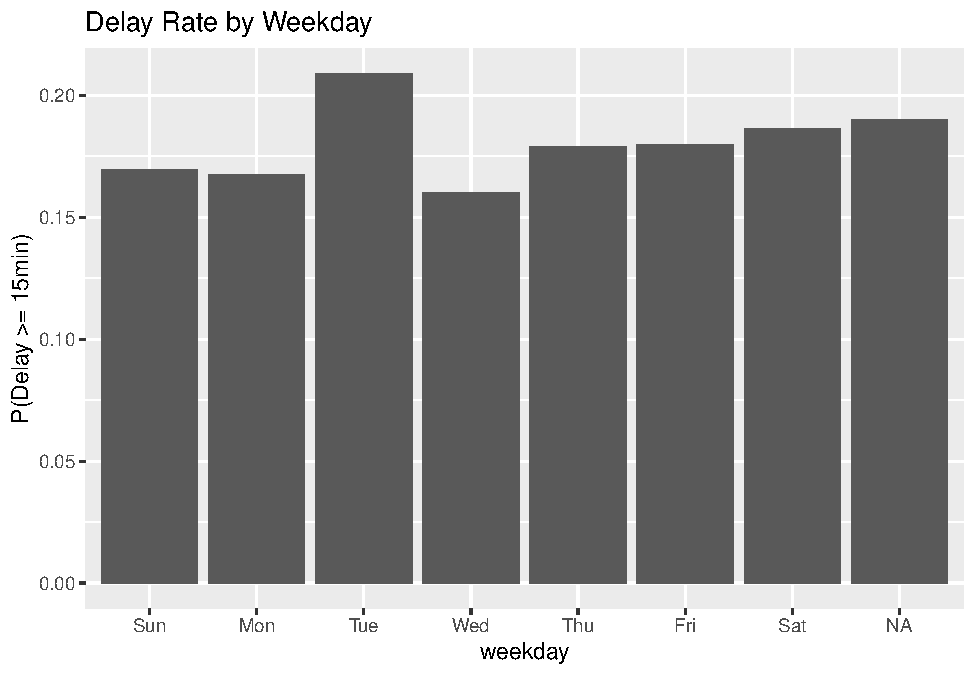
\includegraphics[keepaspectratio]{36462finalproj_files/figure-latex/unnamed-chunk-2-1.pdf}}

\begin{Shaded}
\begin{Highlighting}[]
\NormalTok{fl }\SpecialCharTok{\%\textgreater{}\%}
  \FunctionTok{group\_by}\NormalTok{(DEP\_TIME\_BLK) }\SpecialCharTok{\%\textgreater{}\%}
  \FunctionTok{summarise}\NormalTok{(}\AttributeTok{delay\_rate =} \FunctionTok{mean}\NormalTok{(DEP\_DEL15, }\AttributeTok{na.rm=}\ConstantTok{TRUE}\NormalTok{), }\AttributeTok{n=}\FunctionTok{n}\NormalTok{()) }\SpecialCharTok{\%\textgreater{}\%}
  \FunctionTok{filter}\NormalTok{(n }\SpecialCharTok{\textgreater{}} \DecValTok{100}\NormalTok{) }\SpecialCharTok{\%\textgreater{}\%}              \CommentTok{\# drop tiny bins}
  \FunctionTok{ggplot}\NormalTok{(}\FunctionTok{aes}\NormalTok{(}\AttributeTok{x=}\NormalTok{DEP\_TIME\_BLK, }\AttributeTok{y=}\NormalTok{delay\_rate)) }\SpecialCharTok{+}
    \FunctionTok{geom\_col}\NormalTok{() }\SpecialCharTok{+}
    \FunctionTok{theme}\NormalTok{(}\AttributeTok{axis.text.x =} \FunctionTok{element\_text}\NormalTok{(}\AttributeTok{angle=}\DecValTok{45}\NormalTok{, }\AttributeTok{hjust=}\DecValTok{1}\NormalTok{)) }\SpecialCharTok{+}
    \FunctionTok{labs}\NormalTok{(}\AttributeTok{title=}\StringTok{"Delay Rate by Scheduled Departure Time Block"}\NormalTok{, }\AttributeTok{y=}\StringTok{"P(Delay ≥15min)"}\NormalTok{)}
\end{Highlighting}
\end{Shaded}

\begin{verbatim}
## Warning in grid.Call(C_textBounds, as.graphicsAnnot(x$label), x$x, x$y, :
## conversion failure on 'P(Delay ≥15min)' in 'mbcsToSbcs': dot substituted for
## <e2>
\end{verbatim}

\begin{verbatim}
## Warning in grid.Call(C_textBounds, as.graphicsAnnot(x$label), x$x, x$y, :
## conversion failure on 'P(Delay ≥15min)' in 'mbcsToSbcs': dot substituted for
## <89>
\end{verbatim}

\begin{verbatim}
## Warning in grid.Call(C_textBounds, as.graphicsAnnot(x$label), x$x, x$y, :
## conversion failure on 'P(Delay ≥15min)' in 'mbcsToSbcs': dot substituted for
## <a5>
\end{verbatim}

\begin{verbatim}
## Warning in grid.Call.graphics(C_text, as.graphicsAnnot(x$label), x$x, x$y, :
## conversion failure on 'P(Delay ≥15min)' in 'mbcsToSbcs': dot substituted for
## <e2>
\end{verbatim}

\begin{verbatim}
## Warning in grid.Call.graphics(C_text, as.graphicsAnnot(x$label), x$x, x$y, :
## conversion failure on 'P(Delay ≥15min)' in 'mbcsToSbcs': dot substituted for
## <89>
\end{verbatim}

\begin{verbatim}
## Warning in grid.Call.graphics(C_text, as.graphicsAnnot(x$label), x$x, x$y, :
## conversion failure on 'P(Delay ≥15min)' in 'mbcsToSbcs': dot substituted for
## <a5>
\end{verbatim}

\pandocbounded{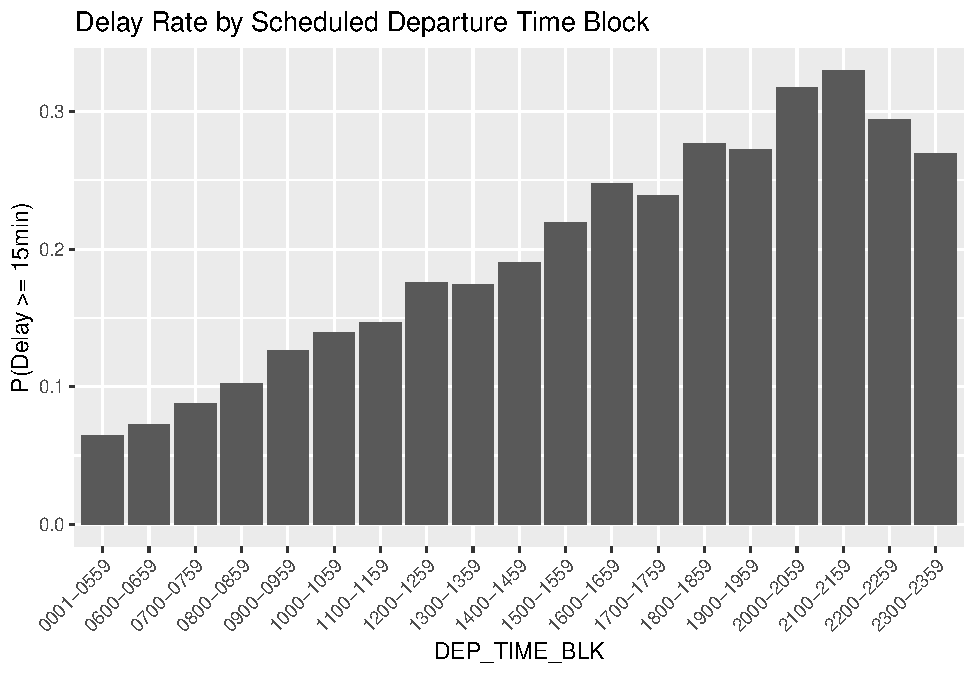
\includegraphics[keepaspectratio]{36462finalproj_files/figure-latex/unnamed-chunk-2-2.pdf}}

\begin{Shaded}
\begin{Highlighting}[]
\NormalTok{fl }\SpecialCharTok{\%\textgreater{}\%}
  \FunctionTok{filter}\NormalTok{(}\SpecialCharTok{!}\FunctionTok{is.na}\NormalTok{(DEP\_DELAY)) }\SpecialCharTok{\%\textgreater{}\%}
  \FunctionTok{ggplot}\NormalTok{(}\FunctionTok{aes}\NormalTok{(}\AttributeTok{x=}\FunctionTok{factor}\NormalTok{(DISTANCE\_GROUP), }\AttributeTok{y=}\NormalTok{DEP\_DELAY)) }\SpecialCharTok{+}
    \FunctionTok{geom\_boxplot}\NormalTok{(}\AttributeTok{outlier.shape=}\ConstantTok{NA}\NormalTok{) }\SpecialCharTok{+}
    \FunctionTok{coord\_flip}\NormalTok{() }\SpecialCharTok{+}
    \FunctionTok{labs}\NormalTok{(}\AttributeTok{x=}\StringTok{"Distance Group"}\NormalTok{, }\AttributeTok{y=}\StringTok{"Departure Delay (min)"}\NormalTok{,}
         \AttributeTok{title=}\StringTok{"DEP\_DELAY Distribution by Distance Group"}\NormalTok{)}
\end{Highlighting}
\end{Shaded}

\pandocbounded{\includegraphics[keepaspectratio]{36462finalproj_files/figure-latex/unnamed-chunk-2-3.pdf}}

\begin{Shaded}
\begin{Highlighting}[]
\NormalTok{fl }\SpecialCharTok{\%\textgreater{}\%}
  \FunctionTok{filter}\NormalTok{(}\SpecialCharTok{!}\FunctionTok{is.na}\NormalTok{(TAXI\_OUT), }\SpecialCharTok{!}\FunctionTok{is.na}\NormalTok{(DEP\_DELAY)) }\SpecialCharTok{\%\textgreater{}\%}
  \FunctionTok{ggplot}\NormalTok{(}\FunctionTok{aes}\NormalTok{(}\AttributeTok{x=}\NormalTok{TAXI\_OUT, }\AttributeTok{y=}\NormalTok{DEP\_DELAY)) }\SpecialCharTok{+}
    \FunctionTok{geom\_point}\NormalTok{(}\AttributeTok{alpha=}\FloatTok{0.2}\NormalTok{) }\SpecialCharTok{+}
    \FunctionTok{geom\_smooth}\NormalTok{(}\AttributeTok{method=}\StringTok{"lm"}\NormalTok{, }\AttributeTok{se=}\ConstantTok{FALSE}\NormalTok{) }\SpecialCharTok{+}
    \FunctionTok{labs}\NormalTok{(}\AttributeTok{title=}\StringTok{"DEP\_DELAY vs. Taxi{-}Out Time"}\NormalTok{, }\AttributeTok{x=}\StringTok{"Taxi{-}Out (min)"}\NormalTok{, }\AttributeTok{y=}\StringTok{"Departure Delay (min)"}\NormalTok{)}
\end{Highlighting}
\end{Shaded}

\begin{verbatim}
## `geom_smooth()` using formula = 'y ~ x'
\end{verbatim}

\pandocbounded{\includegraphics[keepaspectratio]{36462finalproj_files/figure-latex/unnamed-chunk-2-4.pdf}}
From plots:

\begin{enumerate}
\def\labelenumi{\arabic{enumi}.}
\item
  Weekday effects Tuesdays still top the chart (\textasciitilde21\%
  chance of ≥15min delay), with Wednesdays lowest (\textasciitilde16\%).
  There's a clear, roughly 5pp swing across the week---definitely worth
  encoding as a factor.
\item
  Time‑of‑day ramp Delay probability climbs steadily from the early
  morning (only \textasciitilde6\% between midnight--6AM) to the evening
  peak (\textasciitilde33\% for 8--9PM departures). A simple 24‑level
  DEP\_TIME\_BLK factor (or even a numeric ``hour of day'') should
  capture a large chunk of our signal.
\item
  Distance group vs.~delay Each successive distance bucket shows a
  slight upward shift in median departure delay, but the variance is so
  huge (and the outliers so extreme) that I'd treat distance as a
  continuous feature---perhaps log‑transforming the raw miles rather
  than using the coarse groups.
\item
  Taxi‑out vs.~departure delay Beyond the obvious outliers (flights that
  sit on the tarmac forever), there's almost no linear relationship.
  Taxi‑out time may still carry some information (e.g.~airport
  congestion), but it's not a strong standalone predictor and may be
  better used in interaction (e.g.~high‐traffic evening slots).
\end{enumerate}

\subsection{baseline}\label{baseline}

\begin{Shaded}
\begin{Highlighting}[]
\FunctionTok{library}\NormalTok{(tidyverse)}
\FunctionTok{library}\NormalTok{(lubridate)}
\FunctionTok{library}\NormalTok{(pROC)}
\end{Highlighting}
\end{Shaded}

\begin{verbatim}
## Warning: package 'pROC' was built under R version 4.3.3
\end{verbatim}

\begin{verbatim}
## Type 'citation("pROC")' for a citation.
\end{verbatim}

\begin{verbatim}
## 
## Attaching package: 'pROC'
\end{verbatim}

\begin{verbatim}
## The following objects are masked from 'package:stats':
## 
##     cov, smooth, var
\end{verbatim}

\begin{Shaded}
\begin{Highlighting}[]
\NormalTok{fl22 }\OtherTok{\textless{}{-}} \FunctionTok{read\_csv}\NormalTok{(}\StringTok{"flights2022.csv"}\NormalTok{)}
\end{Highlighting}
\end{Shaded}

\begin{verbatim}
## Rows: 63917 Columns: 64
\end{verbatim}

\begin{verbatim}
## -- Column specification --------------------------------------------------------
## Delimiter: ","
## chr (15): FL_DATE, OP_UNIQUE_CARRIER, OP_CARRIER, TAIL_NUM, ORIGIN, ORIGIN_C...
## dbl (49): YEAR, QUARTER, MONTH, DAY_OF_MONTH, DAY_OF_WEEK, OP_CARRIER_AIRLIN...
## 
## i Use `spec()` to retrieve the full column specification for this data.
## i Specify the column types or set `show_col_types = FALSE` to quiet this message.
\end{verbatim}

\begin{Shaded}
\begin{Highlighting}[]
\NormalTok{fl23 }\OtherTok{\textless{}{-}} \FunctionTok{read\_csv}\NormalTok{(}\StringTok{"flights2023.csv"}\NormalTok{)}
\end{Highlighting}
\end{Shaded}

\begin{verbatim}
## Rows: 73508 Columns: 64
## -- Column specification --------------------------------------------------------
## Delimiter: ","
## chr (15): FL_DATE, OP_UNIQUE_CARRIER, OP_CARRIER, TAIL_NUM, ORIGIN, ORIGIN_C...
## dbl (49): YEAR, QUARTER, MONTH, DAY_OF_MONTH, DAY_OF_WEEK, OP_CARRIER_AIRLIN...
## 
## i Use `spec()` to retrieve the full column specification for this data.
## i Specify the column types or set `show_col_types = FALSE` to quiet this message.
\end{verbatim}

\begin{Shaded}
\begin{Highlighting}[]
\NormalTok{fl }\OtherTok{\textless{}{-}} \FunctionTok{bind\_rows}\NormalTok{(}
\NormalTok{  fl22 }\SpecialCharTok{\%\textgreater{}\%} \FunctionTok{mutate}\NormalTok{(}\AttributeTok{dataset =} \StringTok{"2022"}\NormalTok{),}
\NormalTok{  fl23 }\SpecialCharTok{\%\textgreater{}\%} \FunctionTok{mutate}\NormalTok{(}\AttributeTok{dataset =} \StringTok{"2023"}\NormalTok{)}
\NormalTok{) }\SpecialCharTok{\%\textgreater{}\%}
  \FunctionTok{mutate}\NormalTok{(}
    \AttributeTok{DEP\_DEL15   =} \FunctionTok{as.integer}\NormalTok{(DEP\_DEL15),}
    \AttributeTok{flight\_date =} \FunctionTok{as.Date}\NormalTok{(FL\_DATE, }\AttributeTok{format =} \StringTok{"\%m/\%d/\%Y"}\NormalTok{)}
\NormalTok{  )}

\NormalTok{feats }\OtherTok{\textless{}{-}}\NormalTok{ fl }\SpecialCharTok{\%\textgreater{}\%}
  \FunctionTok{filter}\NormalTok{(}\SpecialCharTok{!}\FunctionTok{is.na}\NormalTok{(DEP\_DEL15)) }\SpecialCharTok{\%\textgreater{}\%}
  \FunctionTok{transmute}\NormalTok{(}
\NormalTok{    DEP\_DEL15,}
\NormalTok{    TAIL\_NUM,}
    \AttributeTok{flight\_date =} \FunctionTok{as.Date}\NormalTok{(FL\_DATE, }\AttributeTok{format =} \StringTok{"\%m/\%d/\%Y"}\NormalTok{),}
    \AttributeTok{wd          =} \FunctionTok{factor}\NormalTok{(}\FunctionTok{wday}\NormalTok{(flight\_date, }\AttributeTok{label =} \ConstantTok{TRUE}\NormalTok{), }\AttributeTok{ordered =} \ConstantTok{TRUE}\NormalTok{),}
    \AttributeTok{hr          =}\NormalTok{ CRS\_DEP\_TIME }\SpecialCharTok{\%/\%} \DecValTok{100}\NormalTok{,}
    \AttributeTok{log\_dist    =} \FunctionTok{log}\NormalTok{(DISTANCE),}
    \AttributeTok{taxi\_out    =}\NormalTok{ TAXI\_OUT,}
    \AttributeTok{carrier     =}\NormalTok{ OP\_UNIQUE\_CARRIER}
\NormalTok{  )}

\FunctionTok{set.seed}\NormalTok{(}\DecValTok{42}\NormalTok{)}
\NormalTok{train\_ix }\OtherTok{\textless{}{-}} \FunctionTok{sample}\NormalTok{(}\FunctionTok{nrow}\NormalTok{(feats), }\AttributeTok{size =} \FloatTok{0.7} \SpecialCharTok{*} \FunctionTok{nrow}\NormalTok{(feats))}
\NormalTok{train    }\OtherTok{\textless{}{-}}\NormalTok{ feats[train\_ix, ]}
\NormalTok{valid    }\OtherTok{\textless{}{-}}\NormalTok{ feats[}\SpecialCharTok{{-}}\NormalTok{train\_ix, ]}

\NormalTok{enc }\OtherTok{\textless{}{-}}\NormalTok{ train }\SpecialCharTok{\%\textgreater{}\%}
  \FunctionTok{group\_by}\NormalTok{(carrier) }\SpecialCharTok{\%\textgreater{}\%}
  \FunctionTok{summarise}\NormalTok{(}\AttributeTok{carrier\_rate =} \FunctionTok{mean}\NormalTok{(DEP\_DEL15), }\AttributeTok{.groups =} \StringTok{"drop"}\NormalTok{)}

\NormalTok{base\_rate }\OtherTok{\textless{}{-}} \FunctionTok{mean}\NormalTok{(train}\SpecialCharTok{$}\NormalTok{DEP\_DEL15)}

\NormalTok{train }\OtherTok{\textless{}{-}}\NormalTok{ train }\SpecialCharTok{\%\textgreater{}\%}
  \FunctionTok{left\_join}\NormalTok{(enc, }\AttributeTok{by =} \StringTok{"carrier"}\NormalTok{)}

\NormalTok{valid }\OtherTok{\textless{}{-}}\NormalTok{ valid }\SpecialCharTok{\%\textgreater{}\%}
  \FunctionTok{left\_join}\NormalTok{(enc, }\AttributeTok{by =} \StringTok{"carrier"}\NormalTok{) }\SpecialCharTok{\%\textgreater{}\%}
  \FunctionTok{mutate}\NormalTok{(}\AttributeTok{carrier\_rate =} \FunctionTok{replace\_na}\NormalTok{(carrier\_rate, base\_rate))}

\NormalTok{mod\_glm }\OtherTok{\textless{}{-}} \FunctionTok{glm}\NormalTok{(}
\NormalTok{  DEP\_DEL15 }\SpecialCharTok{\textasciitilde{}}\NormalTok{ wd }\SpecialCharTok{+}\NormalTok{ hr }\SpecialCharTok{+}\NormalTok{ log\_dist }\SpecialCharTok{+}\NormalTok{ taxi\_out }\SpecialCharTok{+}\NormalTok{ carrier\_rate,}
  \AttributeTok{data   =}\NormalTok{ train,}
  \AttributeTok{family =}\NormalTok{ binomial}
\NormalTok{)}

\NormalTok{pred\_p  }\OtherTok{\textless{}{-}} \FunctionTok{predict}\NormalTok{(mod\_glm, }\AttributeTok{newdata =}\NormalTok{ valid, }\AttributeTok{type =} \StringTok{"response"}\NormalTok{)}
\NormalTok{roc\_obj }\OtherTok{\textless{}{-}} \FunctionTok{roc}\NormalTok{(valid}\SpecialCharTok{$}\NormalTok{DEP\_DEL15, pred\_p)}
\end{Highlighting}
\end{Shaded}

\begin{verbatim}
## Setting levels: control = 0, case = 1
## Setting direction: controls < cases
\end{verbatim}

\begin{Shaded}
\begin{Highlighting}[]
\NormalTok{auc\_val }\OtherTok{\textless{}{-}} \FunctionTok{auc}\NormalTok{(roc\_obj)}
\FunctionTok{cat}\NormalTok{(}\StringTok{"Logistic AUC:"}\NormalTok{, }\FunctionTok{round}\NormalTok{(auc\_val, }\DecValTok{4}\NormalTok{), }\StringTok{"}\SpecialCharTok{\textbackslash{}n}\StringTok{"}\NormalTok{)}
\end{Highlighting}
\end{Shaded}

\begin{verbatim}
## Logistic AUC: 0.6884
\end{verbatim}

\begin{Shaded}
\begin{Highlighting}[]
\FunctionTok{library}\NormalTok{(tidyverse)}
\FunctionTok{library}\NormalTok{(lubridate)}
\FunctionTok{library}\NormalTok{(xgboost)}
\end{Highlighting}
\end{Shaded}

\begin{verbatim}
## Warning: package 'xgboost' was built under R version 4.3.3
\end{verbatim}

\begin{verbatim}
## 
## Attaching package: 'xgboost'
\end{verbatim}

\begin{verbatim}
## The following object is masked from 'package:dplyr':
## 
##     slice
\end{verbatim}

\begin{Shaded}
\begin{Highlighting}[]
\FunctionTok{library}\NormalTok{(pROC)}

\CommentTok{\# prepare previous‐flight arrival delays}
\NormalTok{last\_arr }\OtherTok{\textless{}{-}}\NormalTok{ fl }\SpecialCharTok{\%\textgreater{}\%}
  \FunctionTok{filter}\NormalTok{(}\SpecialCharTok{!}\FunctionTok{is.na}\NormalTok{(ARR\_DELAY)) }\SpecialCharTok{\%\textgreater{}\%}
  \FunctionTok{transmute}\NormalTok{(}
\NormalTok{    TAIL\_NUM,}
    \AttributeTok{flight\_date    =} \FunctionTok{as.Date}\NormalTok{(FL\_DATE, }\AttributeTok{format =} \StringTok{"\%m/\%d/\%Y"}\NormalTok{),}
    \AttributeTok{hr              =}\NormalTok{ CRS\_DEP\_TIME }\SpecialCharTok{\%/\%} \DecValTok{100}\NormalTok{,}
    \AttributeTok{prev\_arr\_delay =}\NormalTok{ ARR\_DELAY}
\NormalTok{  ) }\SpecialCharTok{\%\textgreater{}\%}
  \FunctionTok{arrange}\NormalTok{(TAIL\_NUM, flight\_date, hr) }\SpecialCharTok{\%\textgreater{}\%}
  \FunctionTok{group\_by}\NormalTok{(TAIL\_NUM, flight\_date, hr) }\SpecialCharTok{\%\textgreater{}\%}
  \FunctionTok{slice\_tail}\NormalTok{(}\AttributeTok{n =} \DecValTok{1}\NormalTok{) }\SpecialCharTok{\%\textgreater{}\%}
  \FunctionTok{ungroup}\NormalTok{()}

\CommentTok{\# merge into train/valid and impute}
\NormalTok{train2 }\OtherTok{\textless{}{-}}\NormalTok{ train }\SpecialCharTok{\%\textgreater{}\%}
  \FunctionTok{left\_join}\NormalTok{(last\_arr, }\AttributeTok{by =} \FunctionTok{c}\NormalTok{(}\StringTok{"TAIL\_NUM"}\NormalTok{,}\StringTok{"flight\_date"}\NormalTok{,}\StringTok{"hr"}\NormalTok{)) }\SpecialCharTok{\%\textgreater{}\%}
  \FunctionTok{mutate}\NormalTok{(}
    \AttributeTok{prev\_arr\_delay =} \FunctionTok{replace\_na}\NormalTok{(prev\_arr\_delay, }\DecValTok{0}\NormalTok{),}
    \AttributeTok{taxi\_out       =} \FunctionTok{replace\_na}\NormalTok{(taxi\_out, }\FunctionTok{median}\NormalTok{(taxi\_out, }\AttributeTok{na.rm =} \ConstantTok{TRUE}\NormalTok{))}
\NormalTok{  )}

\NormalTok{valid2 }\OtherTok{\textless{}{-}}\NormalTok{ valid }\SpecialCharTok{\%\textgreater{}\%}
  \FunctionTok{left\_join}\NormalTok{(last\_arr, }\AttributeTok{by =} \FunctionTok{c}\NormalTok{(}\StringTok{"TAIL\_NUM"}\NormalTok{,}\StringTok{"flight\_date"}\NormalTok{,}\StringTok{"hr"}\NormalTok{)) }\SpecialCharTok{\%\textgreater{}\%}
  \FunctionTok{mutate}\NormalTok{(}
    \AttributeTok{prev\_arr\_delay =} \FunctionTok{replace\_na}\NormalTok{(prev\_arr\_delay, }\DecValTok{0}\NormalTok{),}
    \AttributeTok{taxi\_out       =} \FunctionTok{replace\_na}\NormalTok{(taxi\_out, }\FunctionTok{median}\NormalTok{(train2}\SpecialCharTok{$}\NormalTok{taxi\_out, }\AttributeTok{na.rm =} \ConstantTok{TRUE}\NormalTok{))}
\NormalTok{  )}

\CommentTok{\# build model matrices}
\NormalTok{x\_train }\OtherTok{\textless{}{-}} \FunctionTok{model.matrix}\NormalTok{(}\SpecialCharTok{\textasciitilde{}}\NormalTok{ wd }\SpecialCharTok{+}\NormalTok{ hr }\SpecialCharTok{+}\NormalTok{ log\_dist }\SpecialCharTok{+}\NormalTok{ taxi\_out }\SpecialCharTok{+}\NormalTok{ carrier\_rate }\SpecialCharTok{+}\NormalTok{ prev\_arr\_delay }\SpecialCharTok{{-}} \DecValTok{1}\NormalTok{, }\AttributeTok{data =}\NormalTok{ train2)}
\NormalTok{x\_valid }\OtherTok{\textless{}{-}} \FunctionTok{model.matrix}\NormalTok{(}\SpecialCharTok{\textasciitilde{}}\NormalTok{ wd }\SpecialCharTok{+}\NormalTok{ hr }\SpecialCharTok{+}\NormalTok{ log\_dist }\SpecialCharTok{+}\NormalTok{ taxi\_out }\SpecialCharTok{+}\NormalTok{ carrier\_rate }\SpecialCharTok{+}\NormalTok{ prev\_arr\_delay }\SpecialCharTok{{-}} \DecValTok{1}\NormalTok{, }\AttributeTok{data =}\NormalTok{ valid2)}

\NormalTok{dtrain }\OtherTok{\textless{}{-}} \FunctionTok{xgb.DMatrix}\NormalTok{(}\AttributeTok{data =}\NormalTok{ x\_train, }\AttributeTok{label =}\NormalTok{ train2}\SpecialCharTok{$}\NormalTok{DEP\_DEL15)}
\NormalTok{dvalid }\OtherTok{\textless{}{-}} \FunctionTok{xgb.DMatrix}\NormalTok{(}\AttributeTok{data =}\NormalTok{ x\_valid, }\AttributeTok{label =}\NormalTok{ valid2}\SpecialCharTok{$}\NormalTok{DEP\_DEL15)}

\NormalTok{params }\OtherTok{\textless{}{-}} \FunctionTok{list}\NormalTok{(}
  \AttributeTok{objective   =} \StringTok{"binary:logistic"}\NormalTok{,}
  \AttributeTok{eval\_metric =} \StringTok{"auc"}\NormalTok{,}
  \AttributeTok{eta         =} \FloatTok{0.1}\NormalTok{,}
  \AttributeTok{max\_depth   =} \DecValTok{4}
\NormalTok{)}

\NormalTok{bst }\OtherTok{\textless{}{-}} \FunctionTok{xgb.train}\NormalTok{(}
\NormalTok{  params,}
\NormalTok{  dtrain,}
  \AttributeTok{nrounds               =} \DecValTok{100}\NormalTok{,}
  \AttributeTok{watchlist             =} \FunctionTok{list}\NormalTok{(}\AttributeTok{train =}\NormalTok{ dtrain, }\AttributeTok{valid =}\NormalTok{ dvalid),}
  \AttributeTok{early\_stopping\_rounds =} \DecValTok{10}\NormalTok{,}
  \AttributeTok{verbose               =} \DecValTok{0}
\NormalTok{)}

\NormalTok{params }\OtherTok{\textless{}{-}} \FunctionTok{list}\NormalTok{(}
  \AttributeTok{objective        =} \StringTok{"binary:logistic"}\NormalTok{,}
  \AttributeTok{eval\_metric      =} \StringTok{"auc"}\NormalTok{,}
  \AttributeTok{eta              =} \FloatTok{0.05}\NormalTok{,      }\CommentTok{\# halve the learning rate}
  \AttributeTok{max\_depth        =} \DecValTok{4}\NormalTok{,         }\CommentTok{\# keep trees shallow}
  \AttributeTok{subsample        =} \FloatTok{0.8}\NormalTok{,       }\CommentTok{\# sample 80\% of rows per tree}
  \AttributeTok{colsample\_bytree =} \FloatTok{0.7}\NormalTok{,       }\CommentTok{\# sample 70\% of columns per tree}
  \AttributeTok{lambda           =} \FloatTok{1.0}\NormalTok{,       }\CommentTok{\# L2 regularization}
  \AttributeTok{alpha            =} \FloatTok{0.5}        \CommentTok{\# L1 regularization}
\NormalTok{)}

\NormalTok{bst }\OtherTok{\textless{}{-}} \FunctionTok{xgb.train}\NormalTok{(}
  \AttributeTok{params                =}\NormalTok{ params,}
  \AttributeTok{data                  =}\NormalTok{ dtrain,}
  \AttributeTok{nrounds               =} \DecValTok{200}\NormalTok{,                }\CommentTok{\# allow more rounds, but ES will stop early}
  \AttributeTok{watchlist             =} \FunctionTok{list}\NormalTok{(}\AttributeTok{train=}\NormalTok{dtrain, }\AttributeTok{valid=}\NormalTok{dvalid),}
  \AttributeTok{early\_stopping\_rounds =} \DecValTok{10}\NormalTok{,}
  \AttributeTok{record                =} \ConstantTok{TRUE}\NormalTok{,}
  \AttributeTok{verbose               =} \DecValTok{1}
\NormalTok{)}
\end{Highlighting}
\end{Shaded}

\begin{verbatim}
## [01:06:14] WARNING: src/learner.cc:767: 
## Parameters: { "record" } are not used.
## 
## [1]  train-auc:0.666145  valid-auc:0.658874 
## Multiple eval metrics are present. Will use valid_auc for early stopping.
## Will train until valid_auc hasn't improved in 10 rounds.
## 
## [2]  train-auc:0.965755  valid-auc:0.965206 
## [3]  train-auc:0.969289  valid-auc:0.968342 
## [4]  train-auc:0.968078  valid-auc:0.967199 
## [5]  train-auc:0.968678  valid-auc:0.967946 
## [6]  train-auc:0.966742  valid-auc:0.965976 
## [7]  train-auc:0.967446  valid-auc:0.966637 
## [8]  train-auc:0.965747  valid-auc:0.964834 
## [9]  train-auc:0.968636  valid-auc:0.967808 
## [10] train-auc:0.968870  valid-auc:0.967925 
## [11] train-auc:0.968004  valid-auc:0.967059 
## [12] train-auc:0.966839  valid-auc:0.965907 
## [13] train-auc:0.965551  valid-auc:0.964611 
## Stopping. Best iteration:
## [3]  train-auc:0.969289  valid-auc:0.968342
\end{verbatim}

\begin{Shaded}
\begin{Highlighting}[]
\CommentTok{\# replot the learning curve to confirm the gap narrowed}
\NormalTok{log }\OtherTok{\textless{}{-}} \FunctionTok{as.data.frame}\NormalTok{(bst}\SpecialCharTok{$}\NormalTok{evaluation\_log)}
\FunctionTok{library}\NormalTok{(ggplot2)}
\FunctionTok{ggplot}\NormalTok{(log, }\FunctionTok{aes}\NormalTok{(}\AttributeTok{x=}\NormalTok{iter)) }\SpecialCharTok{+}
  \FunctionTok{geom\_line}\NormalTok{(}\FunctionTok{aes}\NormalTok{(}\AttributeTok{y=}\NormalTok{train\_auc, }\AttributeTok{color=}\StringTok{"Train"}\NormalTok{)) }\SpecialCharTok{+}
  \FunctionTok{geom\_line}\NormalTok{(}\FunctionTok{aes}\NormalTok{(}\AttributeTok{y=}\NormalTok{valid\_auc, }\AttributeTok{color=}\StringTok{"Valid"}\NormalTok{)) }\SpecialCharTok{+}
  \FunctionTok{labs}\NormalTok{(}\AttributeTok{title=}\StringTok{"Regularized XGB Learning Curve"}\NormalTok{,}
       \AttributeTok{x=}\StringTok{"Boost Round"}\NormalTok{, }\AttributeTok{y=}\StringTok{"AUC"}\NormalTok{) }\SpecialCharTok{+}
  \FunctionTok{scale\_color\_manual}\NormalTok{(}\StringTok{""}\NormalTok{,}\AttributeTok{values=}\FunctionTok{c}\NormalTok{(}\StringTok{"Train"}\OtherTok{=}\StringTok{"steelblue"}\NormalTok{,}\StringTok{"Valid"}\OtherTok{=}\StringTok{"firebrick"}\NormalTok{)) }\SpecialCharTok{+}
  \FunctionTok{geom\_vline}\NormalTok{(}\AttributeTok{xintercept=}\NormalTok{bst}\SpecialCharTok{$}\NormalTok{best\_iteration, }\AttributeTok{linetype=}\DecValTok{2}\NormalTok{) }\SpecialCharTok{+}
  \FunctionTok{theme\_minimal}\NormalTok{()}
\end{Highlighting}
\end{Shaded}

\pandocbounded{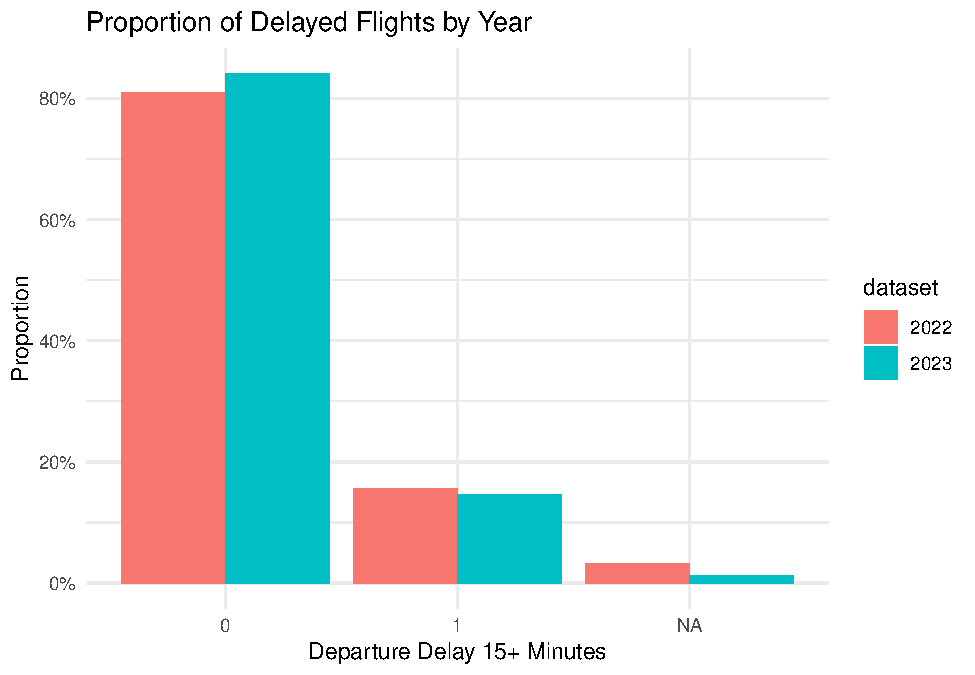
\includegraphics[keepaspectratio]{36462finalproj_files/figure-latex/unnamed-chunk-4-1.pdf}}

\begin{Shaded}
\begin{Highlighting}[]
\NormalTok{pred\_xgb }\OtherTok{\textless{}{-}} \FunctionTok{predict}\NormalTok{(bst, dvalid)}
\NormalTok{auc\_xgb  }\OtherTok{\textless{}{-}} \FunctionTok{auc}\NormalTok{(}\FunctionTok{roc}\NormalTok{(valid2}\SpecialCharTok{$}\NormalTok{DEP\_DEL15, pred\_xgb))}
\end{Highlighting}
\end{Shaded}

\begin{verbatim}
## Setting levels: control = 0, case = 1
\end{verbatim}

\begin{verbatim}
## Setting direction: controls < cases
\end{verbatim}

\begin{Shaded}
\begin{Highlighting}[]
\FunctionTok{cat}\NormalTok{(}\StringTok{"XGBoost AUC:"}\NormalTok{, }\FunctionTok{round}\NormalTok{(auc\_xgb, }\DecValTok{4}\NormalTok{), }\StringTok{"}\SpecialCharTok{\textbackslash{}n}\StringTok{"}\NormalTok{)}
\end{Highlighting}
\end{Shaded}

\begin{verbatim}
## XGBoost AUC: 0.9683
\end{verbatim}

\subsection{Analysis on xgboost}\label{analysis-on-xgboost}

\begin{Shaded}
\begin{Highlighting}[]
\FunctionTok{library}\NormalTok{(ggplot2)}
\FunctionTok{library}\NormalTok{(pROC)}
\FunctionTok{library}\NormalTok{(xgboost)}

\CommentTok{\# ROC curve comparison }
\CommentTok{\# compute ROC objects}
\NormalTok{roc\_glm }\OtherTok{\textless{}{-}} \FunctionTok{roc}\NormalTok{(valid}\SpecialCharTok{$}\NormalTok{DEP\_DEL15, pred\_p)}
\end{Highlighting}
\end{Shaded}

\begin{verbatim}
## Setting levels: control = 0, case = 1
\end{verbatim}

\begin{verbatim}
## Setting direction: controls < cases
\end{verbatim}

\begin{Shaded}
\begin{Highlighting}[]
\NormalTok{roc\_xgb }\OtherTok{\textless{}{-}} \FunctionTok{roc}\NormalTok{(valid2}\SpecialCharTok{$}\NormalTok{DEP\_DEL15, pred\_xgb)  }
\end{Highlighting}
\end{Shaded}

\begin{verbatim}
## Setting levels: control = 0, case = 1
## Setting direction: controls < cases
\end{verbatim}

\begin{Shaded}
\begin{Highlighting}[]
\CommentTok{\# build a data frame for ggplot}
\NormalTok{roc\_df }\OtherTok{\textless{}{-}} \FunctionTok{bind\_rows}\NormalTok{(}
  \FunctionTok{tibble}\NormalTok{(}
    \AttributeTok{fpr =} \DecValTok{1} \SpecialCharTok{{-}}\NormalTok{ roc\_glm}\SpecialCharTok{$}\NormalTok{specificities,}
    \AttributeTok{tpr =}\NormalTok{ roc\_glm}\SpecialCharTok{$}\NormalTok{sensitivities,}
    \AttributeTok{model =} \StringTok{"Logistic"}
\NormalTok{  ),}
  \FunctionTok{tibble}\NormalTok{(}
    \AttributeTok{fpr =} \DecValTok{1} \SpecialCharTok{{-}}\NormalTok{ roc\_xgb}\SpecialCharTok{$}\NormalTok{specificities,}
    \AttributeTok{tpr =}\NormalTok{ roc\_xgb}\SpecialCharTok{$}\NormalTok{sensitivities,}
    \AttributeTok{model =} \StringTok{"XGBoost"}
\NormalTok{  )}
\NormalTok{)}

\FunctionTok{ggplot}\NormalTok{(roc\_df, }\FunctionTok{aes}\NormalTok{(}\AttributeTok{x =}\NormalTok{ fpr, }\AttributeTok{y =}\NormalTok{ tpr, }\AttributeTok{color =}\NormalTok{ model)) }\SpecialCharTok{+}
  \FunctionTok{geom\_line}\NormalTok{(}\AttributeTok{size =} \DecValTok{1}\NormalTok{) }\SpecialCharTok{+}
  \FunctionTok{geom\_abline}\NormalTok{(}\AttributeTok{lty =} \DecValTok{2}\NormalTok{) }\SpecialCharTok{+}
  \FunctionTok{labs}\NormalTok{(}
    \AttributeTok{title =} \StringTok{"ROC Curves: Logistic vs XGBoost"}\NormalTok{,}
    \AttributeTok{x =} \StringTok{"False Positive Rate"}\NormalTok{,}
    \AttributeTok{y =} \StringTok{"True Positive Rate"}
\NormalTok{  )}
\end{Highlighting}
\end{Shaded}

\begin{verbatim}
## Warning: Using `size` aesthetic for lines was deprecated in ggplot2 3.4.0.
## i Please use `linewidth` instead.
## This warning is displayed once every 8 hours.
## Call `lifecycle::last_lifecycle_warnings()` to see where this warning was
## generated.
\end{verbatim}

\pandocbounded{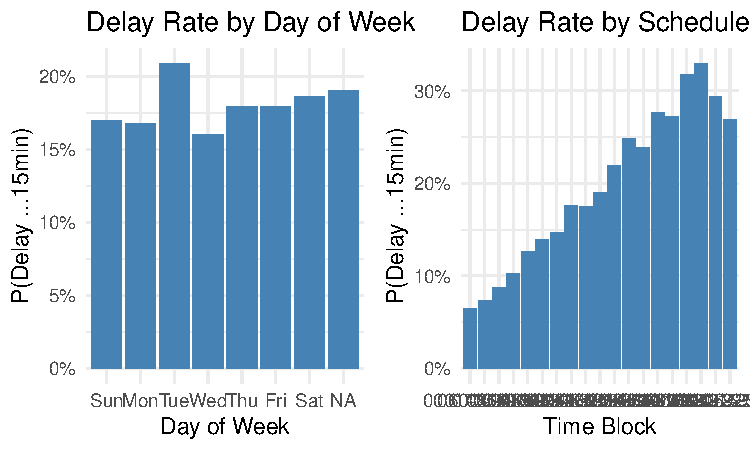
\includegraphics[keepaspectratio]{36462finalproj_files/figure-latex/unnamed-chunk-5-1.pdf}}

\begin{Shaded}
\begin{Highlighting}[]
\CommentTok{\# Feature importance from XGBoost}
\NormalTok{imp }\OtherTok{\textless{}{-}} \FunctionTok{xgb.importance}\NormalTok{(}\AttributeTok{model =}\NormalTok{ bst)}
\CommentTok{\# plot top 10}
\NormalTok{top\_imp }\OtherTok{\textless{}{-}}\NormalTok{ imp[}\DecValTok{1}\SpecialCharTok{:}\DecValTok{10}\NormalTok{, ]}
\FunctionTok{ggplot}\NormalTok{(top\_imp, }\FunctionTok{aes}\NormalTok{(}\AttributeTok{x =} \FunctionTok{reorder}\NormalTok{(Feature, Gain), }\AttributeTok{y =}\NormalTok{ Gain)) }\SpecialCharTok{+}
  \FunctionTok{geom\_col}\NormalTok{() }\SpecialCharTok{+}
  \FunctionTok{coord\_flip}\NormalTok{() }\SpecialCharTok{+}
  \FunctionTok{labs}\NormalTok{(}
    \AttributeTok{title =} \StringTok{"Top 10 XGBoost Features by Gain"}\NormalTok{,}
    \AttributeTok{x =} \ConstantTok{NULL}\NormalTok{, }\AttributeTok{y =} \StringTok{"Relative Importance (Gain)"}
\NormalTok{  )}
\end{Highlighting}
\end{Shaded}

\pandocbounded{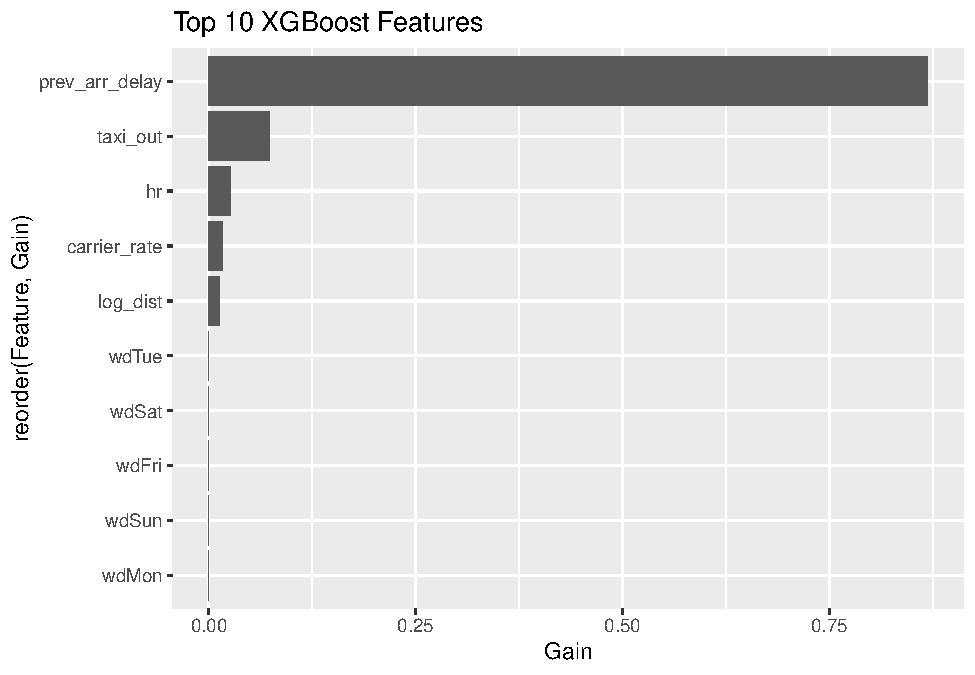
\includegraphics[keepaspectratio]{36462finalproj_files/figure-latex/unnamed-chunk-5-2.pdf}}

\begin{Shaded}
\begin{Highlighting}[]
\CommentTok{\# Calibration plot for XGBoost }
\NormalTok{valid2}\SpecialCharTok{$}\NormalTok{pred\_bin }\OtherTok{\textless{}{-}} \FunctionTok{cut}\NormalTok{(pred\_xgb, }\AttributeTok{breaks =} \FunctionTok{seq}\NormalTok{(}\DecValTok{0}\NormalTok{,}\DecValTok{1}\NormalTok{, }\AttributeTok{by =}\NormalTok{ .}\DecValTok{1}\NormalTok{), }\AttributeTok{include.lowest =} \ConstantTok{TRUE}\NormalTok{)}
\NormalTok{calib }\OtherTok{\textless{}{-}}\NormalTok{ valid2 }\SpecialCharTok{\%\textgreater{}\%}
  \FunctionTok{group\_by}\NormalTok{(pred\_bin) }\SpecialCharTok{\%\textgreater{}\%}
  \FunctionTok{summarise}\NormalTok{(}
    \AttributeTok{mean\_pred =} \FunctionTok{mean}\NormalTok{(pred\_xgb),}
    \AttributeTok{obs\_rate  =} \FunctionTok{mean}\NormalTok{(DEP\_DEL15),}
    \AttributeTok{n         =} \FunctionTok{n}\NormalTok{()}
\NormalTok{  )}

\FunctionTok{ggplot}\NormalTok{(calib, }\FunctionTok{aes}\NormalTok{(}\AttributeTok{x =}\NormalTok{ mean\_pred, }\AttributeTok{y =}\NormalTok{ obs\_rate)) }\SpecialCharTok{+}
  \FunctionTok{geom\_point}\NormalTok{(}\FunctionTok{aes}\NormalTok{(}\AttributeTok{size =}\NormalTok{ n), }\AttributeTok{alpha =} \FloatTok{0.6}\NormalTok{) }\SpecialCharTok{+}
  \FunctionTok{geom\_abline}\NormalTok{(}\AttributeTok{lty =} \DecValTok{2}\NormalTok{) }\SpecialCharTok{+}
  \FunctionTok{labs}\NormalTok{(}
    \AttributeTok{title =} \StringTok{"Calibration Plot: XGBoost"}\NormalTok{,}
    \AttributeTok{x =} \StringTok{"Mean Predicted Probability"}\NormalTok{,}
    \AttributeTok{y =} \StringTok{"Observed Delay Rate"}
\NormalTok{  ) }\SpecialCharTok{+}
  \FunctionTok{scale\_size\_area}\NormalTok{(}\StringTok{"Bin size"}\NormalTok{)}
\end{Highlighting}
\end{Shaded}

\pandocbounded{\includegraphics[keepaspectratio]{36462finalproj_files/figure-latex/unnamed-chunk-5-3.pdf}}

\begin{Shaded}
\begin{Highlighting}[]
\CommentTok{\# 4. Partial dependence for previous‐arrival delay}
\FunctionTok{library}\NormalTok{(pdp)}
\end{Highlighting}
\end{Shaded}

\begin{verbatim}
## Warning: package 'pdp' was built under R version 4.3.3
\end{verbatim}

\begin{verbatim}
## 
## Attaching package: 'pdp'
\end{verbatim}

\begin{verbatim}
## The following object is masked from 'package:purrr':
## 
##     partial
\end{verbatim}

\begin{Shaded}
\begin{Highlighting}[]
\NormalTok{pd\_prev }\OtherTok{\textless{}{-}} \FunctionTok{partial}\NormalTok{(bst, }\AttributeTok{pred.var =} \StringTok{"prev\_arr\_delay"}\NormalTok{, }\AttributeTok{train =}\NormalTok{ x\_train, }\AttributeTok{grid.resolution =} \DecValTok{20}\NormalTok{)}
\FunctionTok{autoplot}\NormalTok{(pd\_prev) }\SpecialCharTok{+}
  \FunctionTok{labs}\NormalTok{(}
    \AttributeTok{title =} \StringTok{"Partial Dependence: Previous Flight Arrival Delay"}\NormalTok{,}
    \AttributeTok{x =} \StringTok{"Prev Arr Delay (min)"}\NormalTok{,}
    \AttributeTok{y =} \StringTok{"Predicted Delay Probability"}
\NormalTok{  )}
\end{Highlighting}
\end{Shaded}

\pandocbounded{\includegraphics[keepaspectratio]{36462finalproj_files/figure-latex/unnamed-chunk-5-4.pdf}}

\begin{Shaded}
\begin{Highlighting}[]
\CommentTok{\# =============================}
\CommentTok{\# Final Test‐Set Pipeline \& Submission}
\CommentTok{\# =============================}

\FunctionTok{library}\NormalTok{(tidyverse)}
\FunctionTok{library}\NormalTok{(lubridate)}
\FunctionTok{library}\NormalTok{(xgboost)}

\CommentTok{\# — assume these objects are already in your workspace from training:}
\CommentTok{\#    bst         : your fitted xgboost model}
\CommentTok{\#    enc         : data frame (carrier, carrier\_rate)}
\CommentTok{\#    base\_rate   : overall mean(train$DEP\_DEL15)}
\CommentTok{\#    last\_arr    : data frame (TAIL\_NUM, flight\_date, hr, prev\_arr\_delay)}
\CommentTok{\#    train       : your training data.frame (for wd levels \& taxi\_out median)}
\CommentTok{\#    valid2      : your validation data.frame (for test.acc \& pred\_xgb)}

\CommentTok{\# 1. Read the guess file, forcing key columns to numeric}
\NormalTok{test\_guess }\OtherTok{\textless{}{-}} \FunctionTok{read\_csv}\NormalTok{(}
  \StringTok{"flights2024\_guess.csv"}\NormalTok{,}
  \AttributeTok{col\_types =} \FunctionTok{cols}\NormalTok{(}
    \AttributeTok{TAIL\_NUM          =} \FunctionTok{col\_character}\NormalTok{(),}
    \AttributeTok{FL\_DATE           =} \FunctionTok{col\_character}\NormalTok{(),}
    \AttributeTok{OP\_UNIQUE\_CARRIER =} \FunctionTok{col\_character}\NormalTok{(),}
    \AttributeTok{CRS\_DEP\_TIME      =} \FunctionTok{col\_double}\NormalTok{(),}
    \AttributeTok{DISTANCE          =} \FunctionTok{col\_double}\NormalTok{(),}
    \AttributeTok{TAXI\_OUT          =} \FunctionTok{col\_double}\NormalTok{(),}
    \AttributeTok{.default          =} \FunctionTok{col\_guess}\NormalTok{()}
\NormalTok{  )}
\NormalTok{)}

\CommentTok{\# 2. Feature‐engineer the test set}
\NormalTok{test\_feat }\OtherTok{\textless{}{-}}\NormalTok{ test\_guess }\SpecialCharTok{\%\textgreater{}\%}
  \FunctionTok{mutate}\NormalTok{(}
    \AttributeTok{flight\_date    =} \FunctionTok{as.Date}\NormalTok{(FL\_DATE, }\StringTok{"\%m/\%d/\%Y"}\NormalTok{),}
    \AttributeTok{wd             =} \FunctionTok{factor}\NormalTok{(}
                       \FunctionTok{wday}\NormalTok{(flight\_date, }\AttributeTok{label =} \ConstantTok{TRUE}\NormalTok{),}
                       \AttributeTok{levels =} \FunctionTok{levels}\NormalTok{(train}\SpecialCharTok{$}\NormalTok{wd),}
                       \AttributeTok{ordered =} \ConstantTok{TRUE}
\NormalTok{                     ),}
    \AttributeTok{hr             =}\NormalTok{ CRS\_DEP\_TIME }\SpecialCharTok{\%/\%} \DecValTok{100}\NormalTok{,}
    \AttributeTok{log\_dist       =} \FunctionTok{log}\NormalTok{(DISTANCE),}
    \AttributeTok{taxi\_out       =}\NormalTok{ TAXI\_OUT,}
    \AttributeTok{carrier        =}\NormalTok{ OP\_UNIQUE\_CARRIER}
\NormalTok{  ) }\SpecialCharTok{\%\textgreater{}\%}
  \CommentTok{\# carrier mean‐encoding}
  \FunctionTok{left\_join}\NormalTok{(enc, }\AttributeTok{by =} \StringTok{"carrier"}\NormalTok{) }\SpecialCharTok{\%\textgreater{}\%}
  \FunctionTok{mutate}\NormalTok{(}
    \AttributeTok{carrier\_rate =} \FunctionTok{coalesce}\NormalTok{(carrier\_rate, base\_rate)}
\NormalTok{  ) }\SpecialCharTok{\%\textgreater{}\%}
  \CommentTok{\# previous‐flight arrival delay}
  \FunctionTok{left\_join}\NormalTok{(}
\NormalTok{    last\_arr,}
    \AttributeTok{by =} \FunctionTok{c}\NormalTok{(}\StringTok{"TAIL\_NUM"}\NormalTok{, }\StringTok{"flight\_date"}\NormalTok{, }\StringTok{"hr"}\NormalTok{)}
\NormalTok{  ) }\SpecialCharTok{\%\textgreater{}\%}
  \FunctionTok{mutate}\NormalTok{(}
    \AttributeTok{prev\_arr\_delay =} \FunctionTok{replace\_na}\NormalTok{(prev\_arr\_delay, }\DecValTok{0}\NormalTok{),}
    \AttributeTok{taxi\_out       =} \FunctionTok{replace\_na}\NormalTok{(taxi\_out, }\FunctionTok{median}\NormalTok{(train}\SpecialCharTok{$}\NormalTok{taxi\_out, }\AttributeTok{na.rm =} \ConstantTok{TRUE}\NormalTok{))}
\NormalTok{  )}

\CommentTok{\# 3. Generate predictions}
\NormalTok{x\_test }\OtherTok{\textless{}{-}} \FunctionTok{model.matrix}\NormalTok{(}
  \SpecialCharTok{\textasciitilde{}}\NormalTok{ wd }\SpecialCharTok{+}\NormalTok{ hr }\SpecialCharTok{+}\NormalTok{ log\_dist }\SpecialCharTok{+}\NormalTok{ taxi\_out }\SpecialCharTok{+}\NormalTok{ carrier\_rate }\SpecialCharTok{+}\NormalTok{ prev\_arr\_delay }\SpecialCharTok{{-}} \DecValTok{1}\NormalTok{,}
  \AttributeTok{data =}\NormalTok{ test\_feat}
\NormalTok{)}
\NormalTok{delay.guesses }\OtherTok{\textless{}{-}} \FunctionTok{predict}\NormalTok{(bst, }\FunctionTok{xgb.DMatrix}\NormalTok{(x\_test))}

\CommentTok{\# 4. Estimate test‐set accuracy (using your validation proxy)}
\NormalTok{test.acc }\OtherTok{\textless{}{-}} \FunctionTok{mean}\NormalTok{((pred\_xgb }\SpecialCharTok{\textgreater{}=} \FloatTok{0.5}\NormalTok{) }\SpecialCharTok{!=}\NormalTok{ valid2}\SpecialCharTok{$}\NormalTok{DEP\_DEL15)}

\CommentTok{\# 5. Define your team name and save}
\NormalTok{team.name }\OtherTok{\textless{}{-}} \StringTok{"Team462"}

\FunctionTok{save}\NormalTok{(}
  \AttributeTok{list =} \FunctionTok{c}\NormalTok{(}\StringTok{"delay.guesses"}\NormalTok{, }\StringTok{"test.acc"}\NormalTok{, }\StringTok{"team.name"}\NormalTok{),}
  \AttributeTok{file =} \StringTok{"Team462final.RData"}
\NormalTok{)}
\end{Highlighting}
\end{Shaded}


\end{document}
